\chapter{Statistical Analysis}\label{sec:statistics}

The signal search is performed using a simultaneous fit to the $m_{\ell^+\ell^-\gamma}$ distribution in the eight event categories.
The fit uses a binned maximum likelihood method in the range $105 < m_{\ell^+\ell^-\gamma} < 170$\GeV.
In each category, a likelihood function is defined using analytic models of signal and background events, along with nuisance parameters for systematic uncertainties.
The combined likelihood function is the product of the likelihood functions in each category.
The parameter of interest in the maximum likelihood fit is the signal strength $\mu$, defined as the product of the cross section and the branching fraction [$\sigma(\Pp\Pp\to\PH)\mathcal{B}(\PH\to\PZ\gamma)$], relative to the SM expectation.

\section{Signal Modeling}

The signal model is defined as the sum of Crystal Ball~\cite{CB-Oreglia} and Gaussian functions.
The signal shape parameters are determined by fitting this model to simulated signal events in each category.
To account for differences in mass resolution, these fits are performed separately for the event samples used to model each data-taking year, as well as for muon and electron channel events.
This results in six signal models that are summed to give the total expected signal in a given category.
Table~\ref{tab:yield} gives these mass resolutions for \hzg{}, summed over the three years, as obtained from simulation. The mass resolutions range from 1.4--2.3\GeV, depending on the category.
Separate sets of parameter values are found by fitting simulated events with $m_\PH$ of $120$, $125$, and $130$\GeV.
Using linear interpolation, parameter values are also determined at 1\GeV intervals in $m_\PH$ from $120$--$130$\GeV, as well as at \mH\GeV. 
In the fit to data, the mean and resolution parameters are allowed to vary subject to constraints from several systematic uncertainties, described in Section~\ref{sec:uncertainties}, while the remaining parameters are held fixed.

Figure~\ref{fig:elesigfit} (\ref{fig:musigfit}) shows the signal fits for the $m_\PH=125\GeV$ simulated samples in the electron (muon) channel for the 2016 data-taking period. Figure~\ref{fig:elemusigfit} shows the signal fits for the lepton-tagged category for the 2016 data-taking period, in which electron and muon channel events are combined. In the lepton-tagged category, the signal shape is modeled separately for ZH and WH production in order to account for differences in potential lepton mispairing. Signal fits for the full set of data-taking periods are shown in Appendix~\ref{appendix_signal_fits}.

\begin{figure}
	\begin{center}
		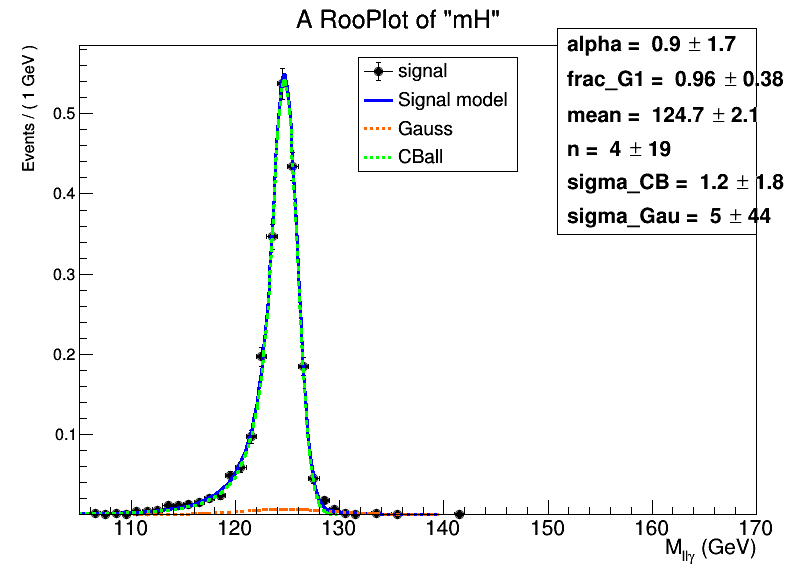
\includegraphics[width=0.40\textwidth]{fig/signal_fit/2016/sigfit_ele_ggF_1_125.png}
		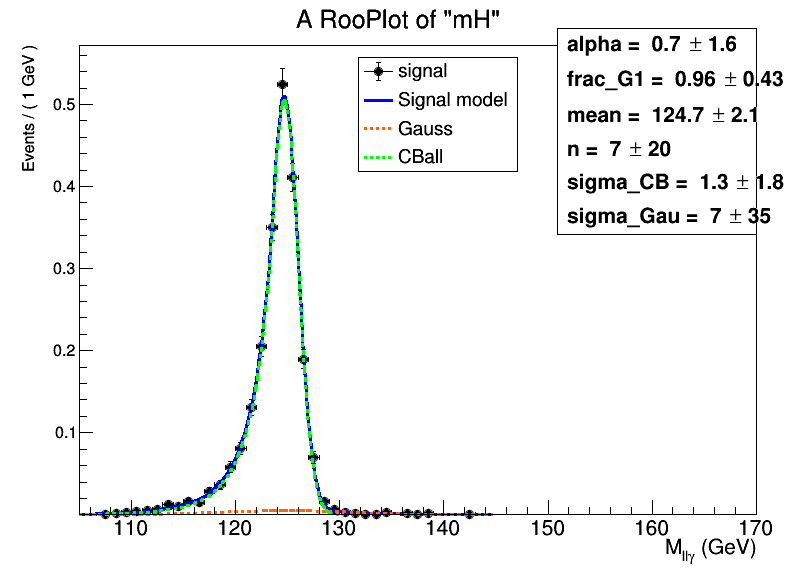
\includegraphics[width=0.40\textwidth]{fig/signal_fit/2016/sigfit_ele_ggF_2_125.png}\\
		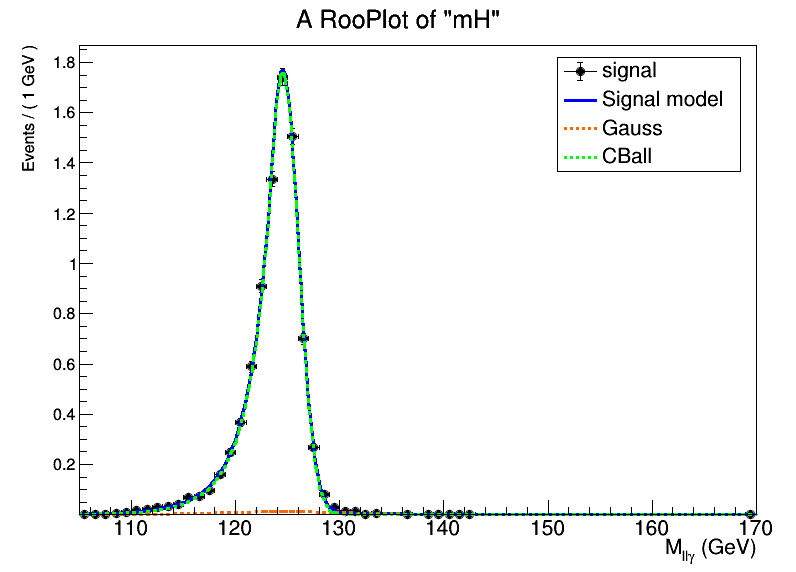
\includegraphics[width=0.40\textwidth]{fig/signal_fit/2016/sigfit_ele_ggF_3_125.png}
		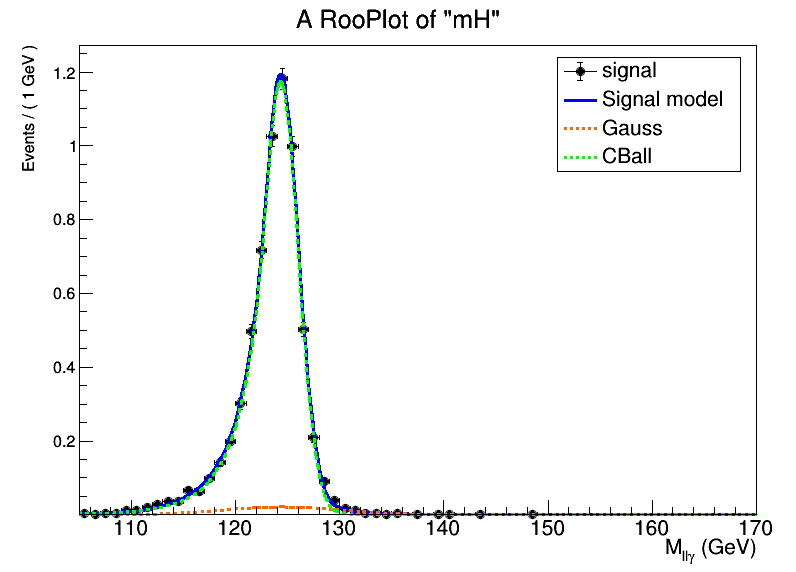
\includegraphics[width=0.40\textwidth]{fig/signal_fit/2016/sigfit_ele_ggF_4_125.png}\\
		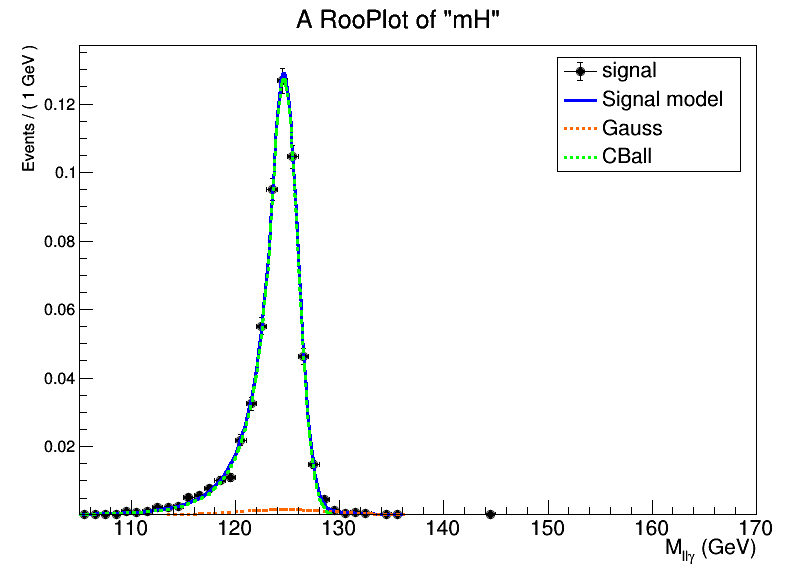
\includegraphics[width=0.40\textwidth]{fig/signal_fit/2016/sigfit_ele_VBF_501_125.png}
		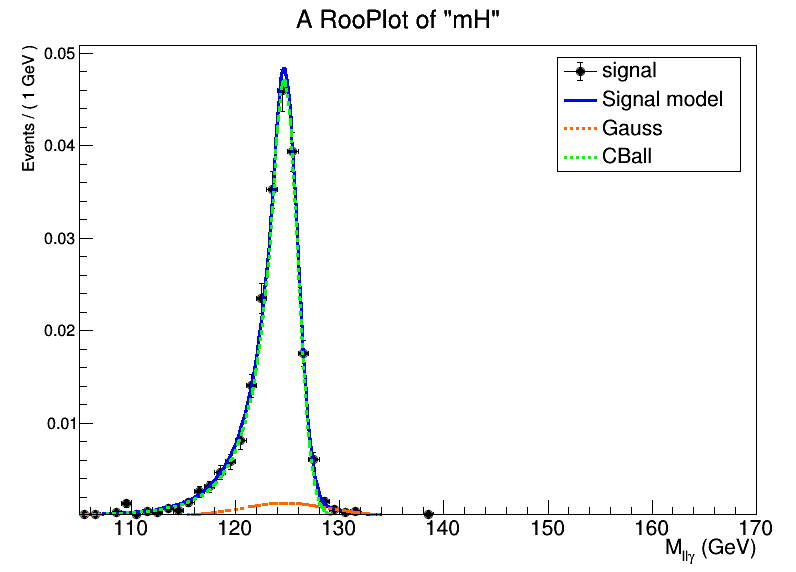
\includegraphics[width=0.40\textwidth]{fig/signal_fit/2016/sigfit_ele_VBF_502_125.png}\\
		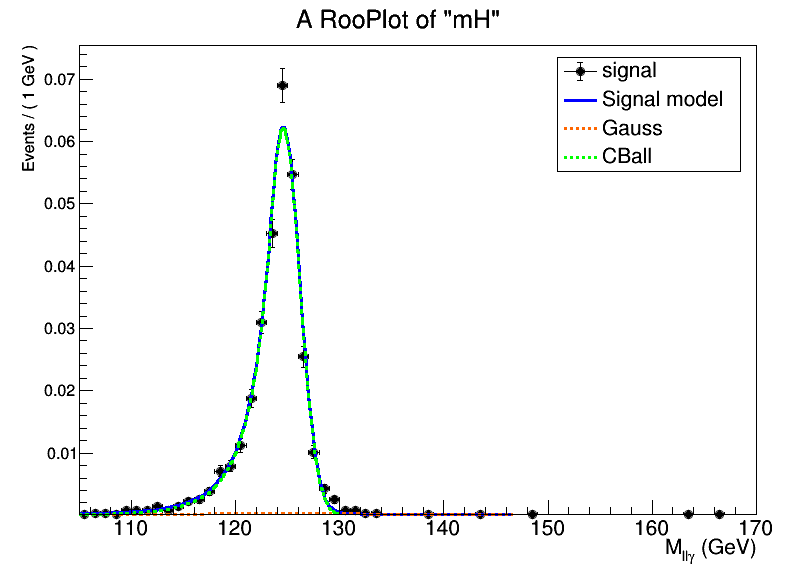
\includegraphics[width=0.40\textwidth]{fig/signal_fit/2016/sigfit_ele_VBF_503_125.png}\\
		\caption{Fits to simulated $m_{\ell^+\ell^-\gamma}$ signal distributions in the electron channel for
            		 $m_\PH=125\GeV$ for the 2016 data-taking period.
			 The blue line shows the total fit function, the green line shows the Crystal Ball function component, and the red line shows the Gaussian function component.
			 The top four plots correspond to the untagged categories, and the bottom three plots correspond to the dijet categories.}
		\label{fig:elesigfit}
	\end{center}
\end{figure}

\begin{figure}
	\begin{center}
		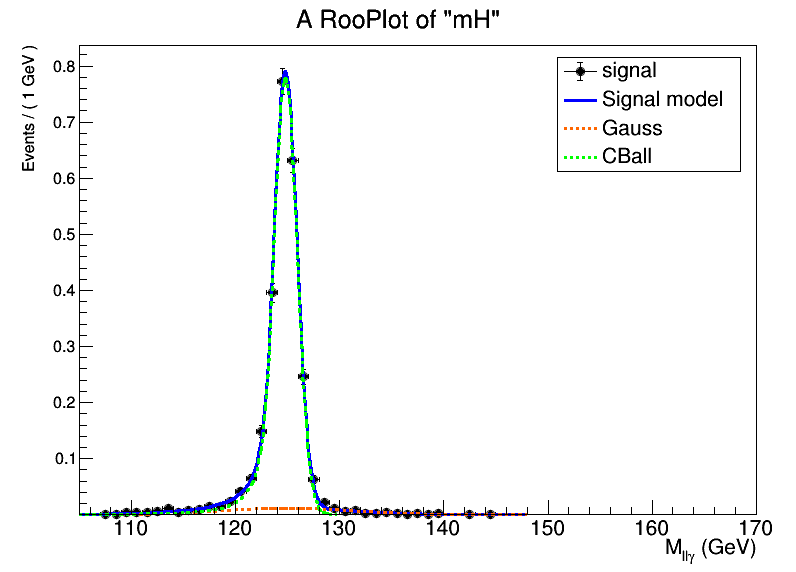
\includegraphics[width=0.40\textwidth]{fig/signal_fit/2016/sigfit_mu_ggF_1_125.png}
		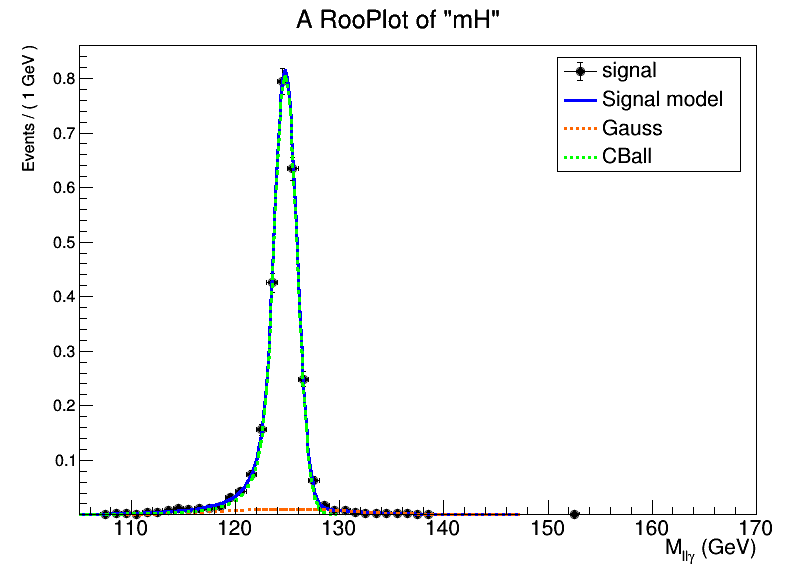
\includegraphics[width=0.40\textwidth]{fig/signal_fit/2016/sigfit_mu_ggF_2_125.png}\\
		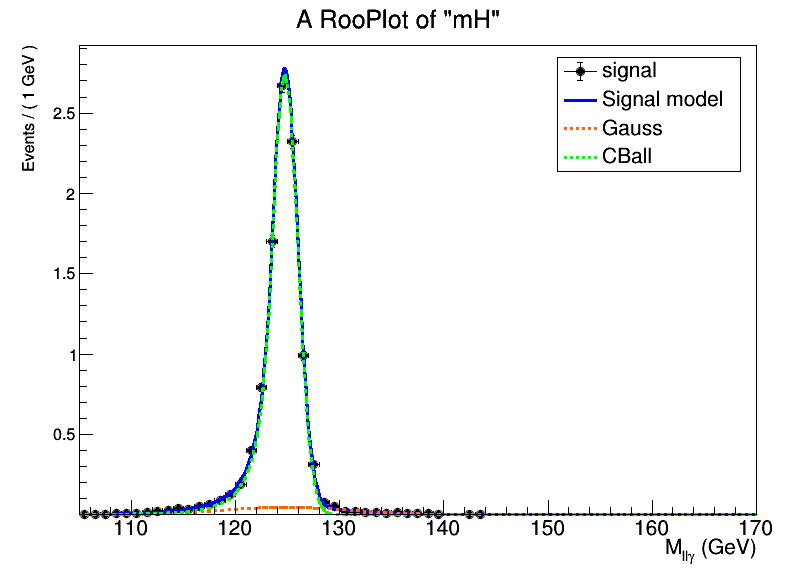
\includegraphics[width=0.40\textwidth]{fig/signal_fit/2016/sigfit_mu_ggF_3_125.png}
		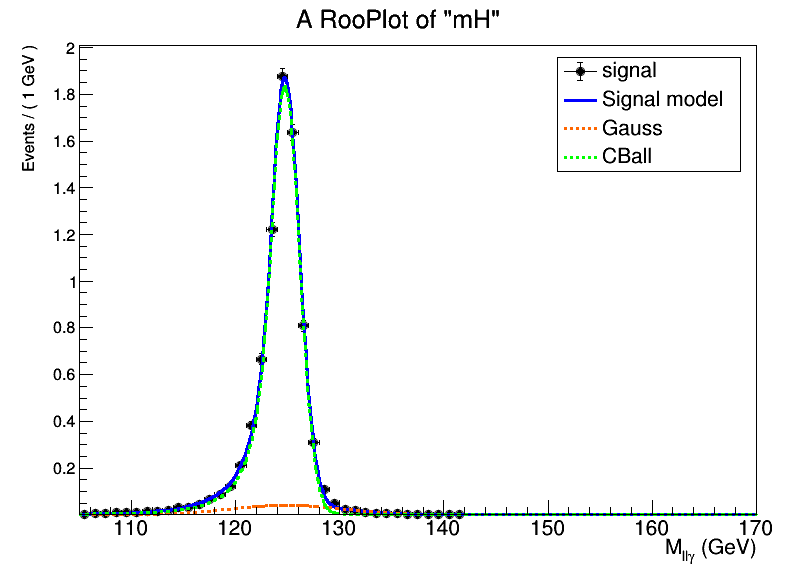
\includegraphics[width=0.40\textwidth]{fig/signal_fit/2016/sigfit_mu_ggF_4_125.png}\\
		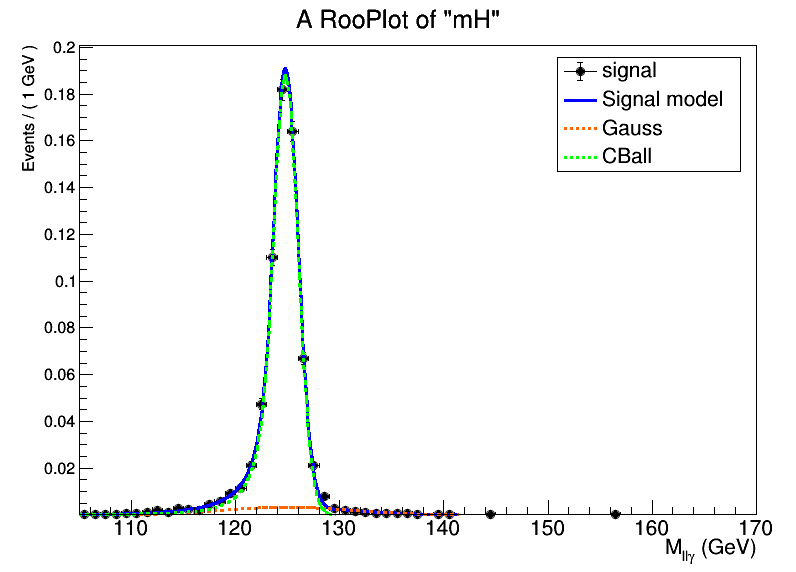
\includegraphics[width=0.40\textwidth]{fig/signal_fit/2016/sigfit_mu_VBF_501_125.png}
		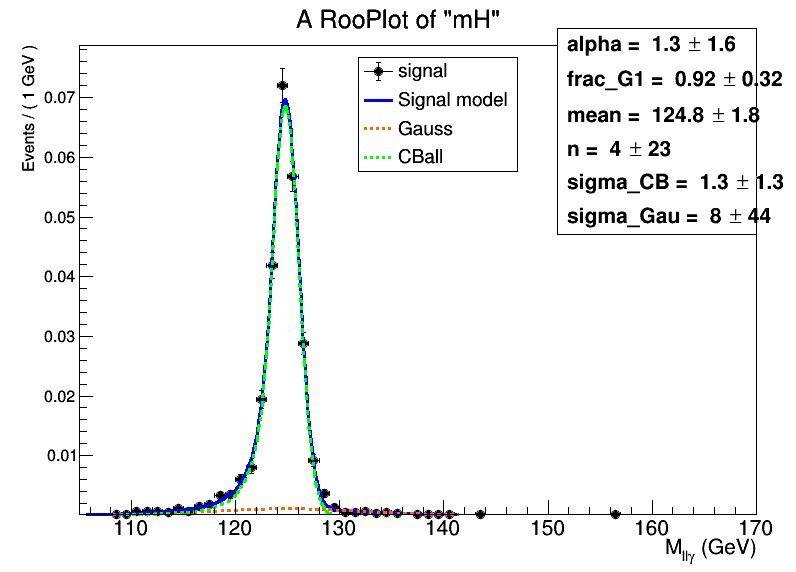
\includegraphics[width=0.40\textwidth]{fig/signal_fit/2016/sigfit_mu_VBF_502_125.png}\\
		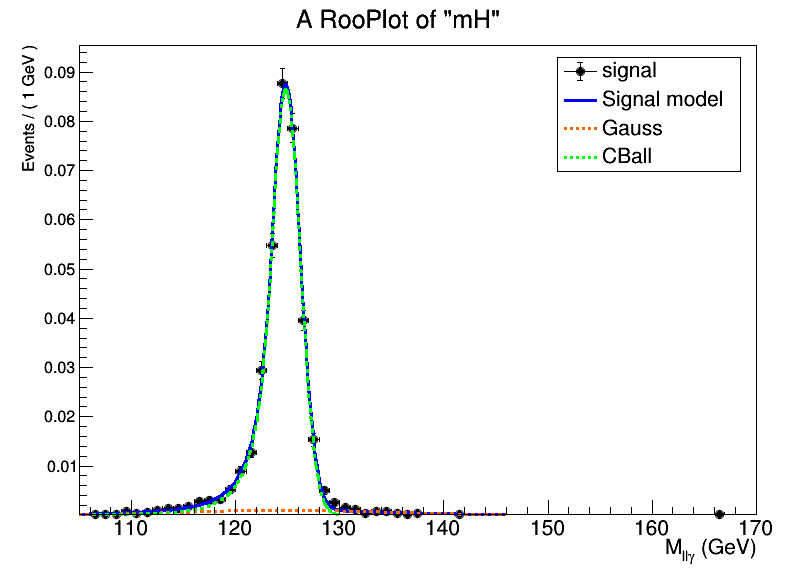
\includegraphics[width=0.40\textwidth]{fig/signal_fit/2016/sigfit_mu_VBF_503_125.png}\\
		\caption{Fits to simulated $m_{\ell^+\ell^-\gamma}$ signal distributions in the muon channel for
            		 $m_\PH=125\GeV$ for the 2016 data-taking period.
			 The blue line shows the total fit function, the green line shows the Crystal Ball function component, and the red line shows the Gaussian function component.
			 The top four plots correspond to the untagged categories, and the bottom three plots correspond to the dijet categories.}
		\label{fig:musigfit}
	\end{center}
\end{figure}

\begin{figure}
	\begin{center}
	  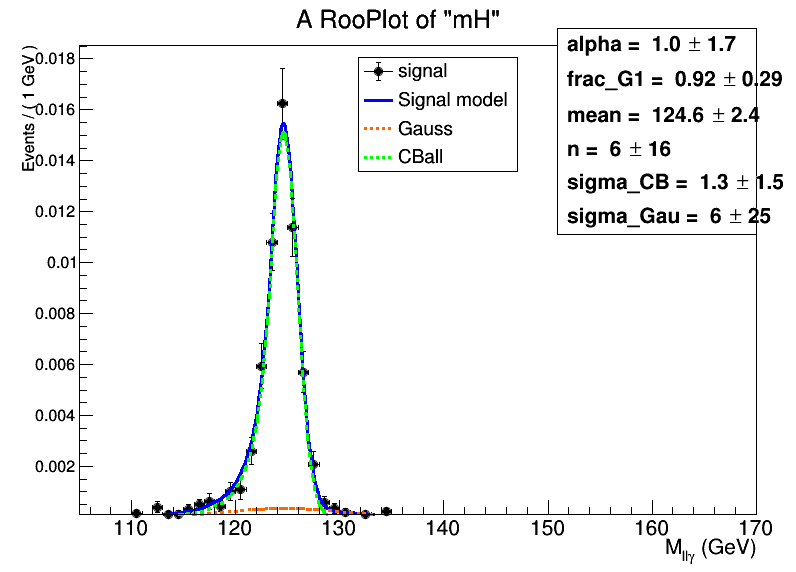
\includegraphics[width=0.40\textwidth]{fig/signal_fit/2016/sigfit_ele_mu_ZH_6789_125.png}
	  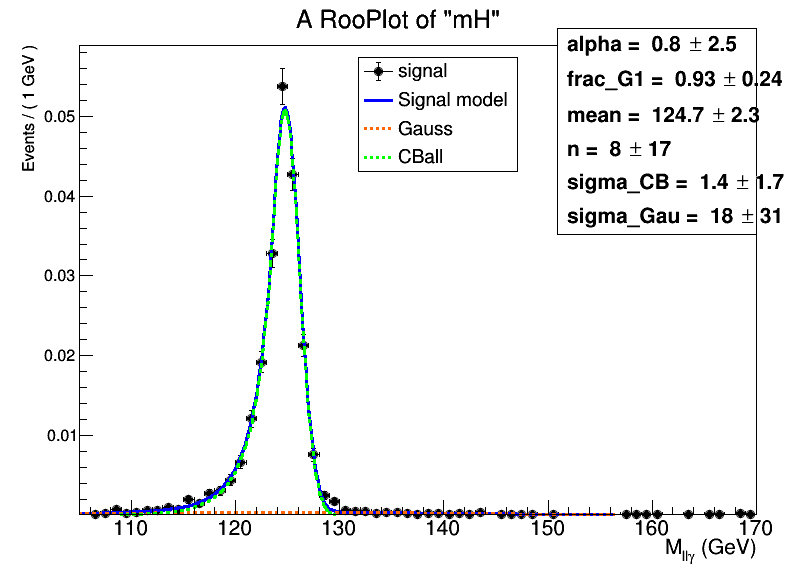
\includegraphics[width=0.40\textwidth]{fig/signal_fit/2016/sigfit_ele_mu_WH_6789_125.png}
		\caption{Fits to simulated $m_{\ell^+\ell^-\gamma}$ signal distributions in the electron and muon channels combined in the lepton-tagged category for
            		 $m_\PH=125\GeV$ for the 2016 data-taking period.
        		 The left plot shows the fit to simulated ZH production events, and the right plot shows the fit to simulated WH production events. 
			 The blue line shows the total fit function, the green line shows the Crystal Ball function component, and the red line shows the Gaussian function component.}
		\label{fig:elemusigfit}
	\end{center}
\end{figure}

\section{Resonant Background Modeling}
The process $\PH\to\mpmm$, where at least one muon radiates an FSR photon, is expected to contribute at the 6\% level relative to the \hzg{} signal yield. Because of this, 
we treat it as a resonant background. To model the $\PH\to\mpmm$ shape, we perform fits to the $m_{\lplm\gamma}$ distributions in simulated event samples, following the same 
procedure used for the signal fits described above. As for the signal, the analytic model is taken to be the sum of Crystal Ball and Gaussian functions. The resulting fits are shown 
in Appendix~\ref{sec:appendix_hmumu}. 

\section{Nonresonant Background Modeling}
The nonresonant background model in each category is obtained from the data using the discrete profiling method~\cite{Dauncey:2014xga}.
This technique accounts for the systematic uncertainty associated with choosing an analytic functional form to fit the background.
The background function is chosen from a set of candidate functions via a discrete nuisance parameter in the fit.
These functions are derived from the data in each category, with muon and electron events from all data-taking years combined.
The $m_{\ell^+\ell^-\gamma}$ spectrum consists of a turn-on peak around 110--115\GeV and a monotonically falling spectrum in the high-mass tail, where the turn-on peak is driven by the photon $\pt$ selection.
These features are modeled by the convolution of a Gaussian function, which is used to describe the lower-mass (turn-on) portion of the spectrum, with a step function that is multiplied by one of several functions, which are used to describe the higher-mass (tail) portion of the spectrum.
The complete function has the general form:
\begin{equation}
    \mathcal{F}(m_{\lplm\gamma}; \mu_{\mathrm{G}}, \sigma_{\mathrm{G}}, s, \vec{\alpha}) = \int_{m_\textrm{min}}^{m_\textrm{max}}\mathcal{N}(m_{\lplm\gamma}-t;\mu_{\mathrm{G}},\sigma_{\mathrm{G}})\Theta(t; s)f(t; \vec{\alpha})dt,
\end{equation}
where $t$ is the integration variable for the convolution, $m_\textrm{min}=105\GeV$ and $m_\textrm{max}=170\GeV$ are the limits of integration, $\mathcal{N}(m_{\ell^+\ell^-\gamma}-t;\mu_{\mathrm{G}},\sigma_{\mathrm{G}})$ is the Gaussian function with mean $\mu_{\mathrm{G}}$ and standard deviation $\sigma_{\mathrm{G}}$, $\Theta(t; s)$ is the Heaviside step function with step location $s$, and $f(t; \vec{\alpha})$ is the falling spectrum function with shape parameters $\vec{\alpha}$.

Since the background modeling strategy has been changed several times throughout the history of the CMS \hzg{} searches, 
it is worthwhile to understand the motivation for the current approach. Previously, in the 2016 analysis,
the background was modeled for the $m_{\lplm\gamma}$ range of 115--170\GeV.
The choice to extend the mass range down to 105\GeV was made in order to improve 
the model in the low mass region near the turn-on peak and avoid potential bias.
Figure~\ref{fig:compare_turnon_fits} shows a comparison of fits in each category with and without modeling the turn-on. From the plots, 
it is clear that modeling the turn-on properly yields a better fit around 115 GeV, the previous lower bound of the fit used in the 2016 search. 

\begin{figure}
	\begin{center}
        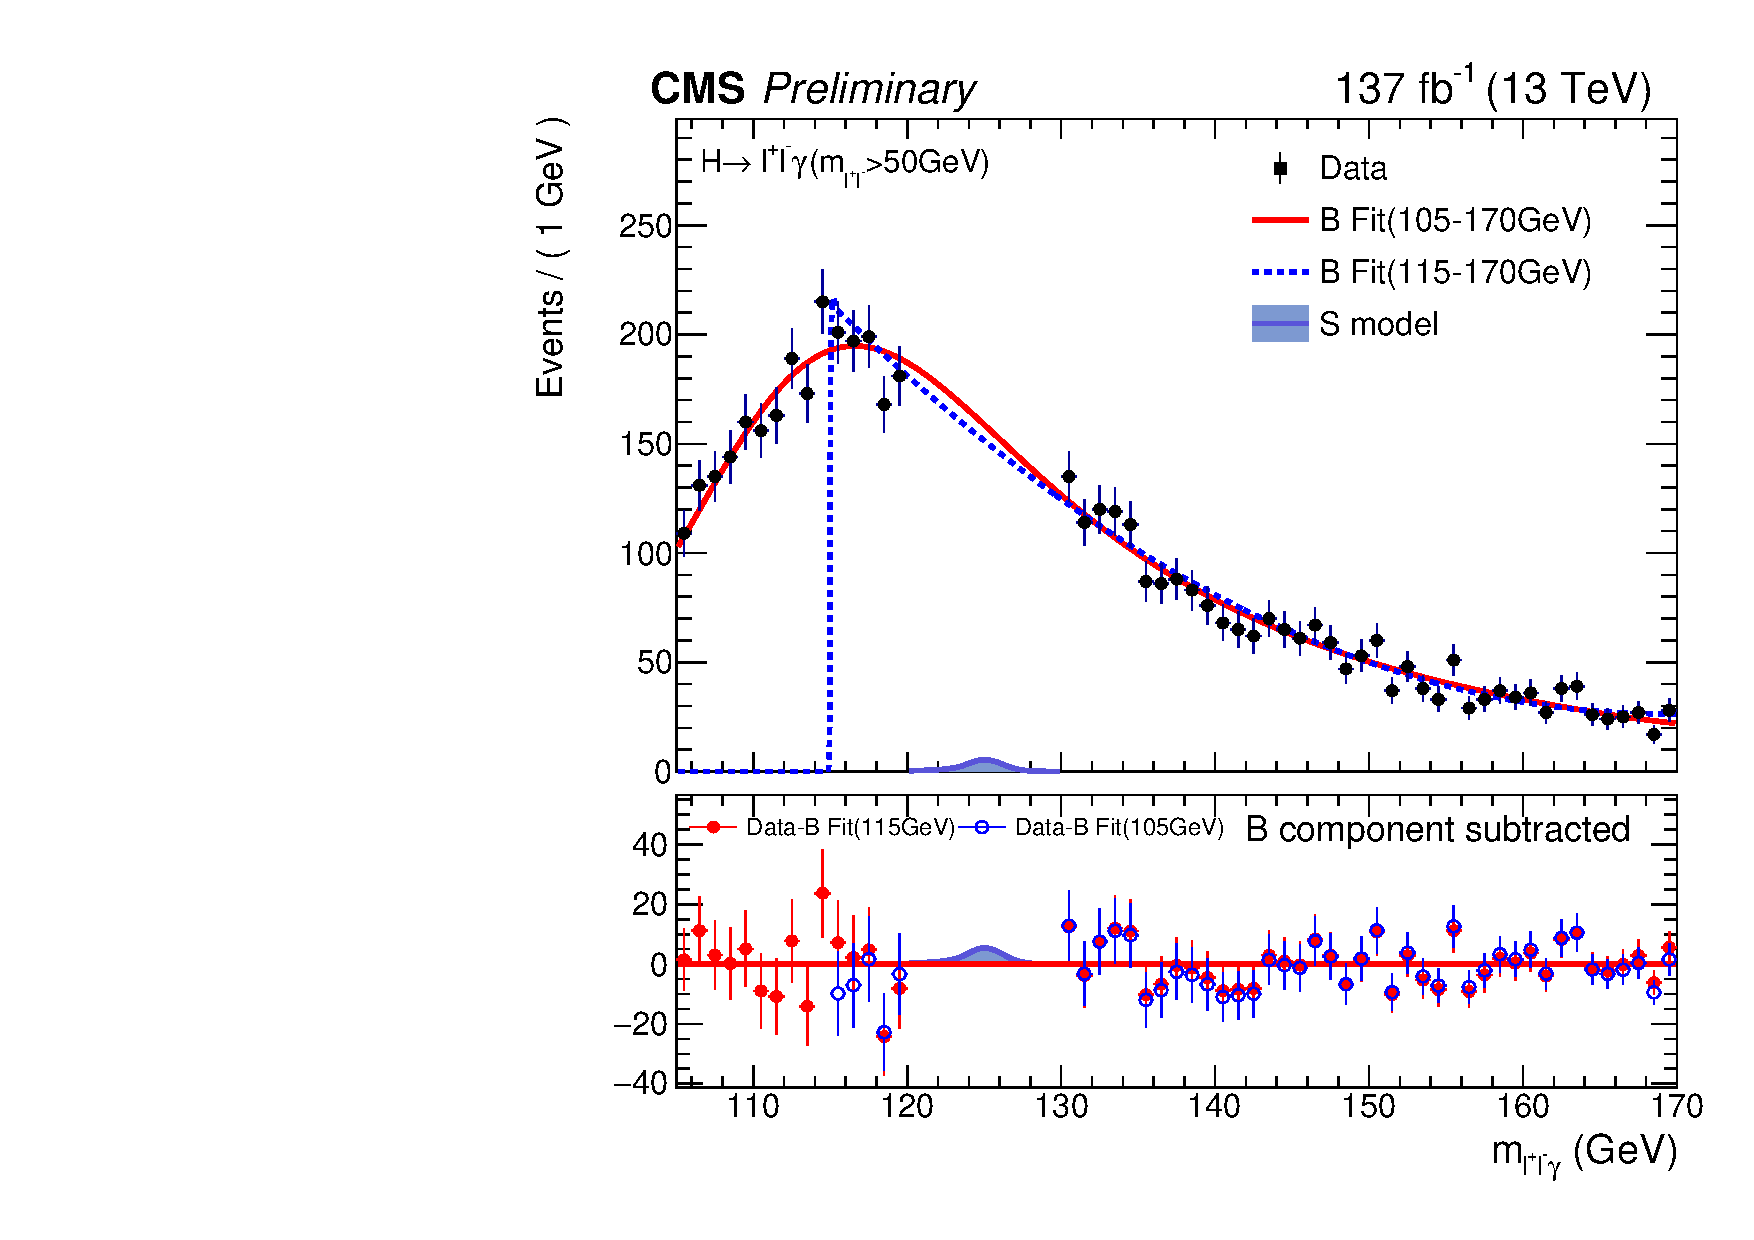
\includegraphics[width=0.27\textwidth]{fig/turnon_comparison/over_cat1_prefit_new.pdf}
        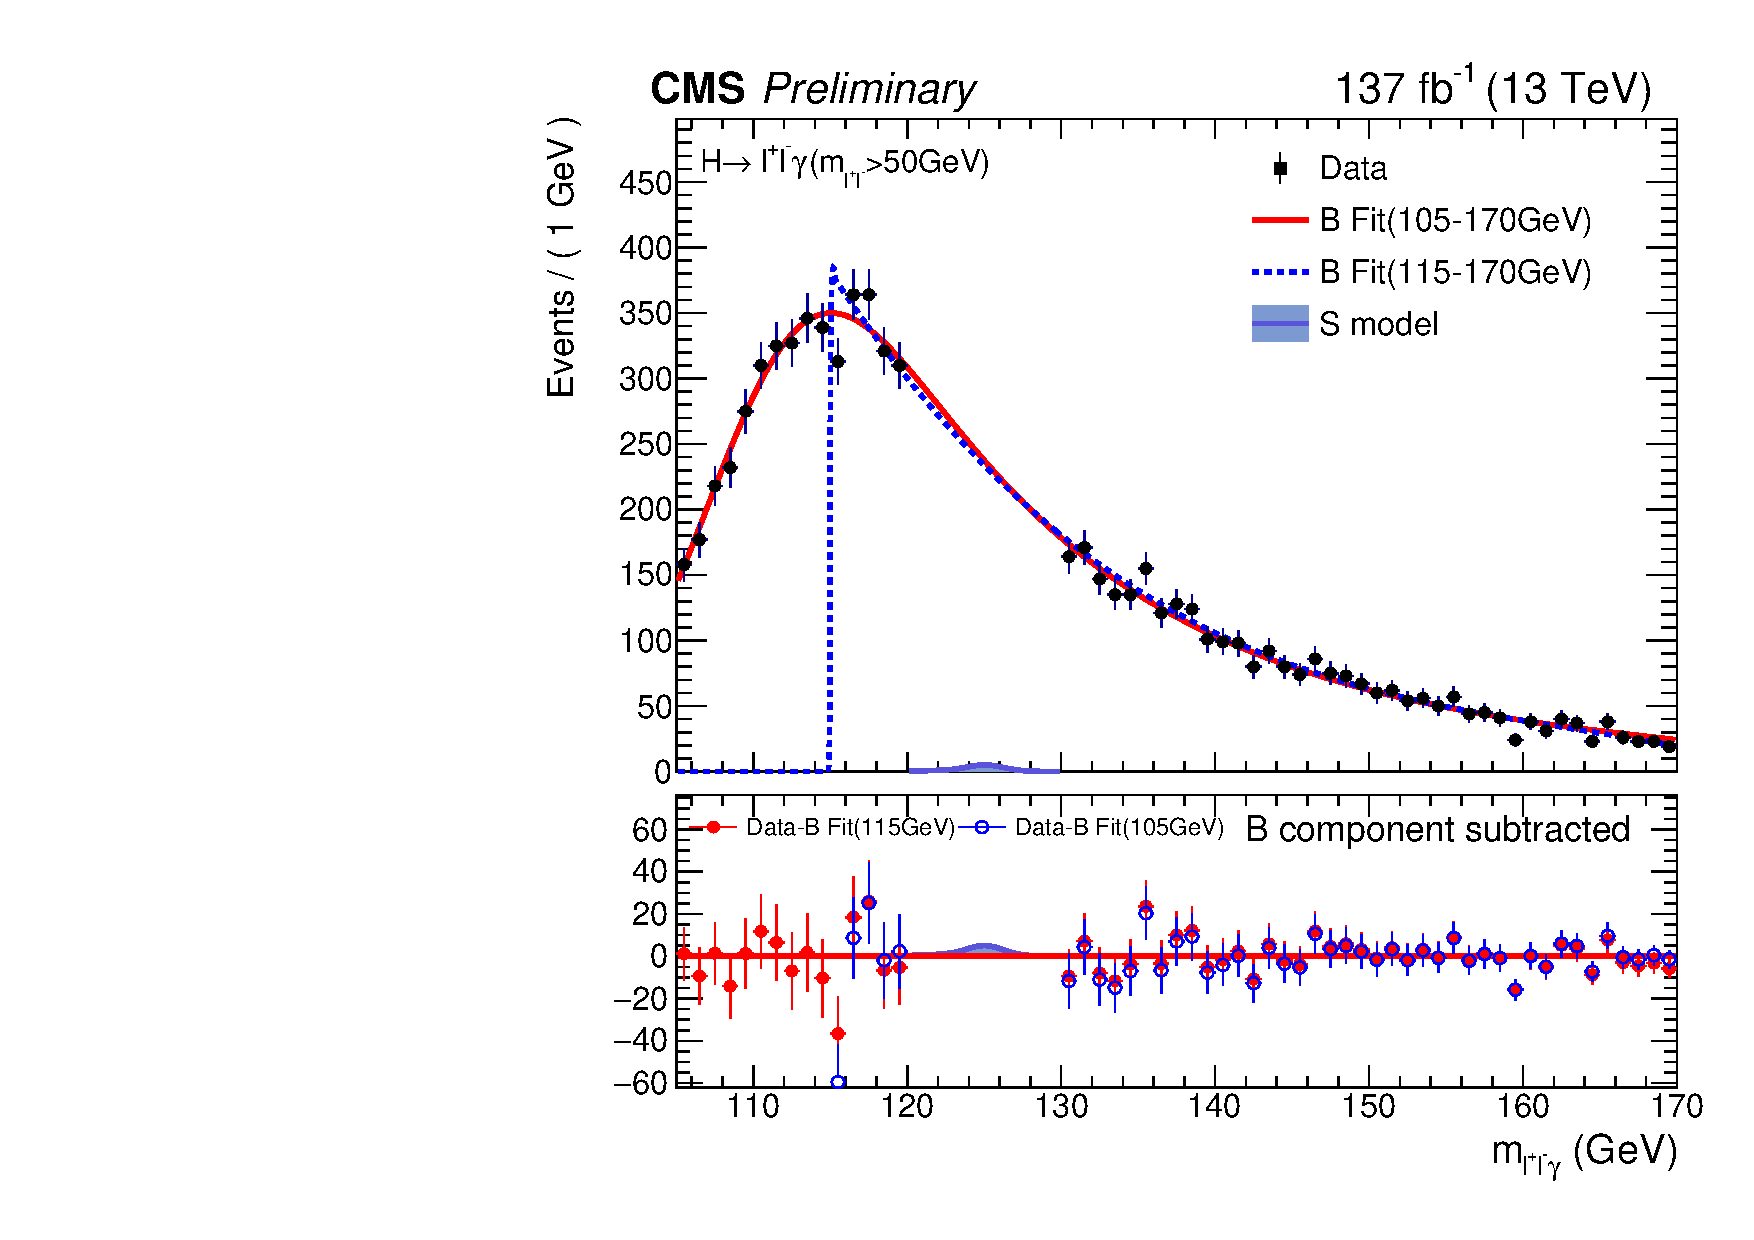
\includegraphics[width=0.27\textwidth]{fig/turnon_comparison/over_cat2_prefit_new.pdf}\\
        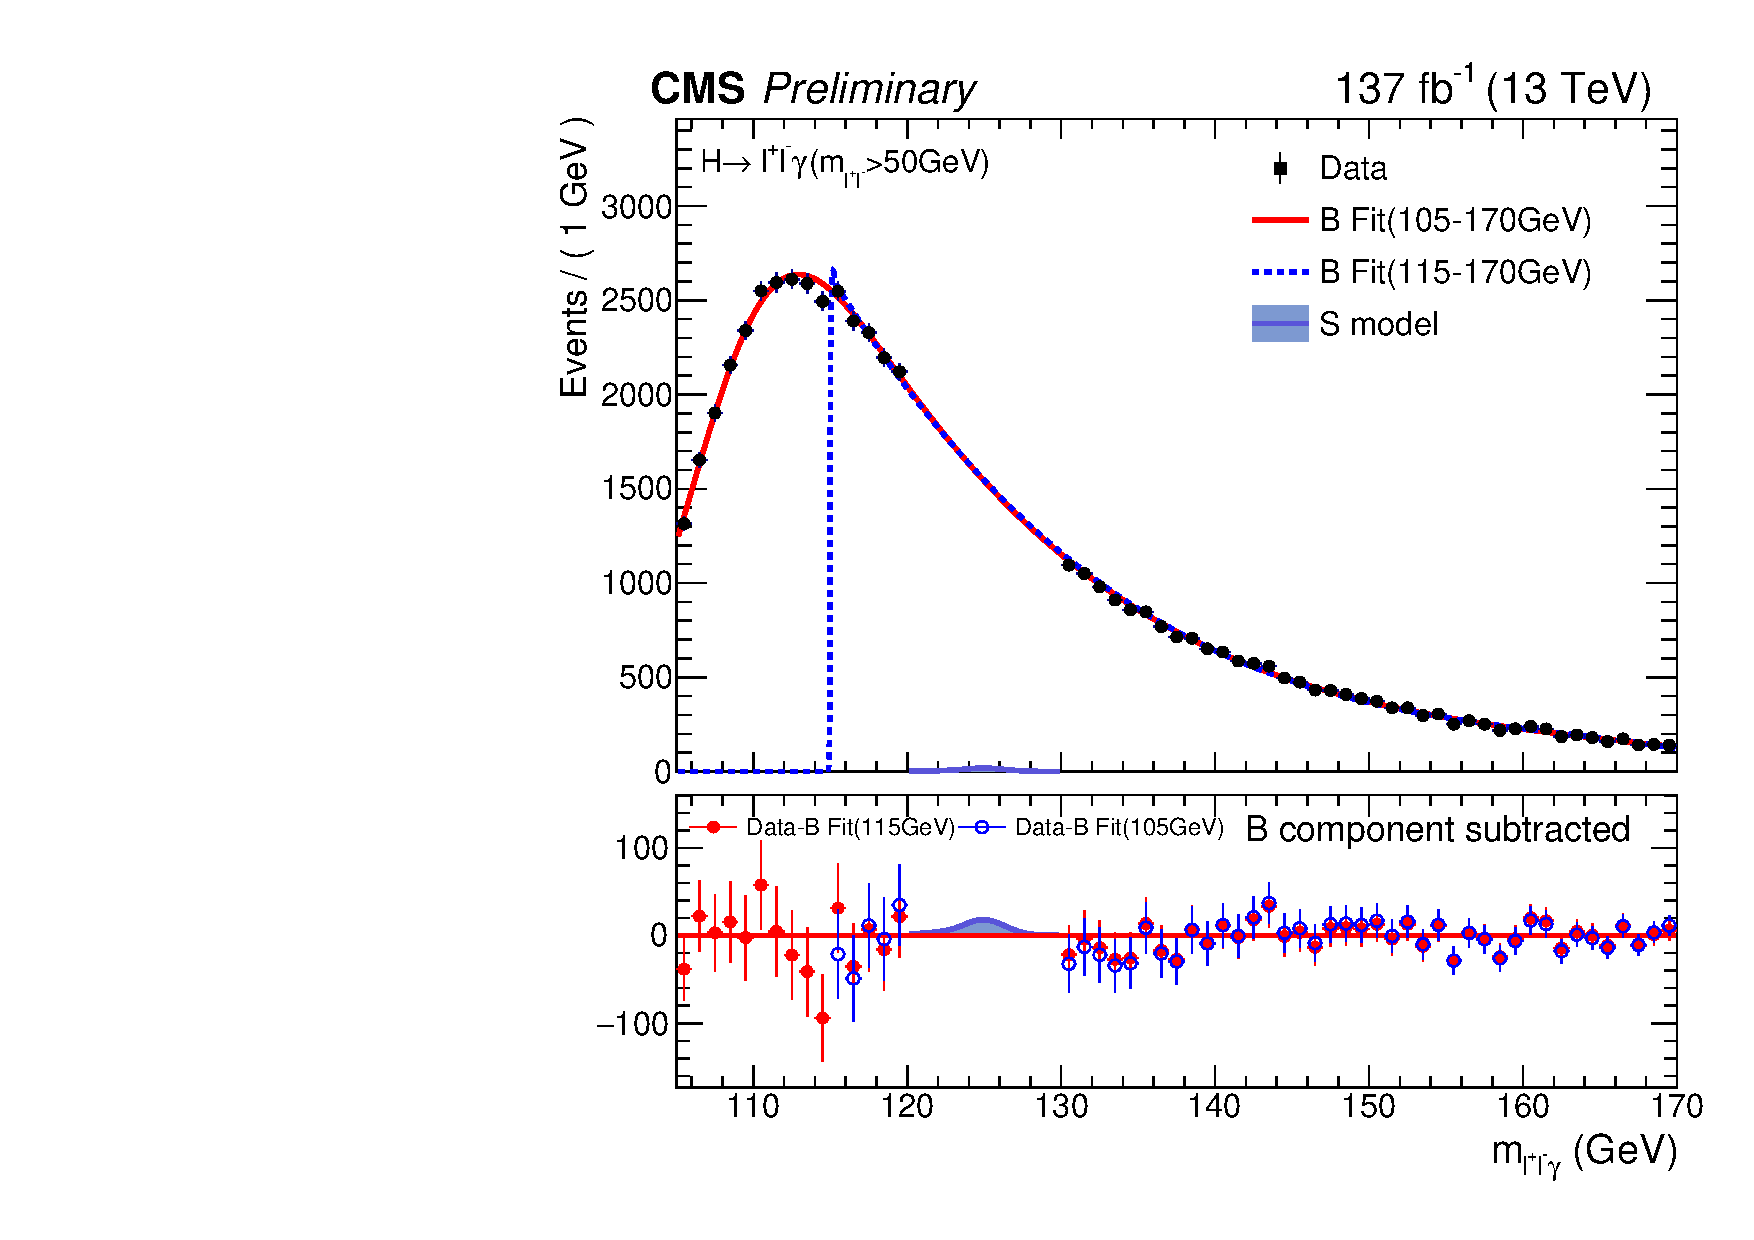
\includegraphics[width=0.27\textwidth]{fig/turnon_comparison/plot_cat3_prefit_new.pdf}
        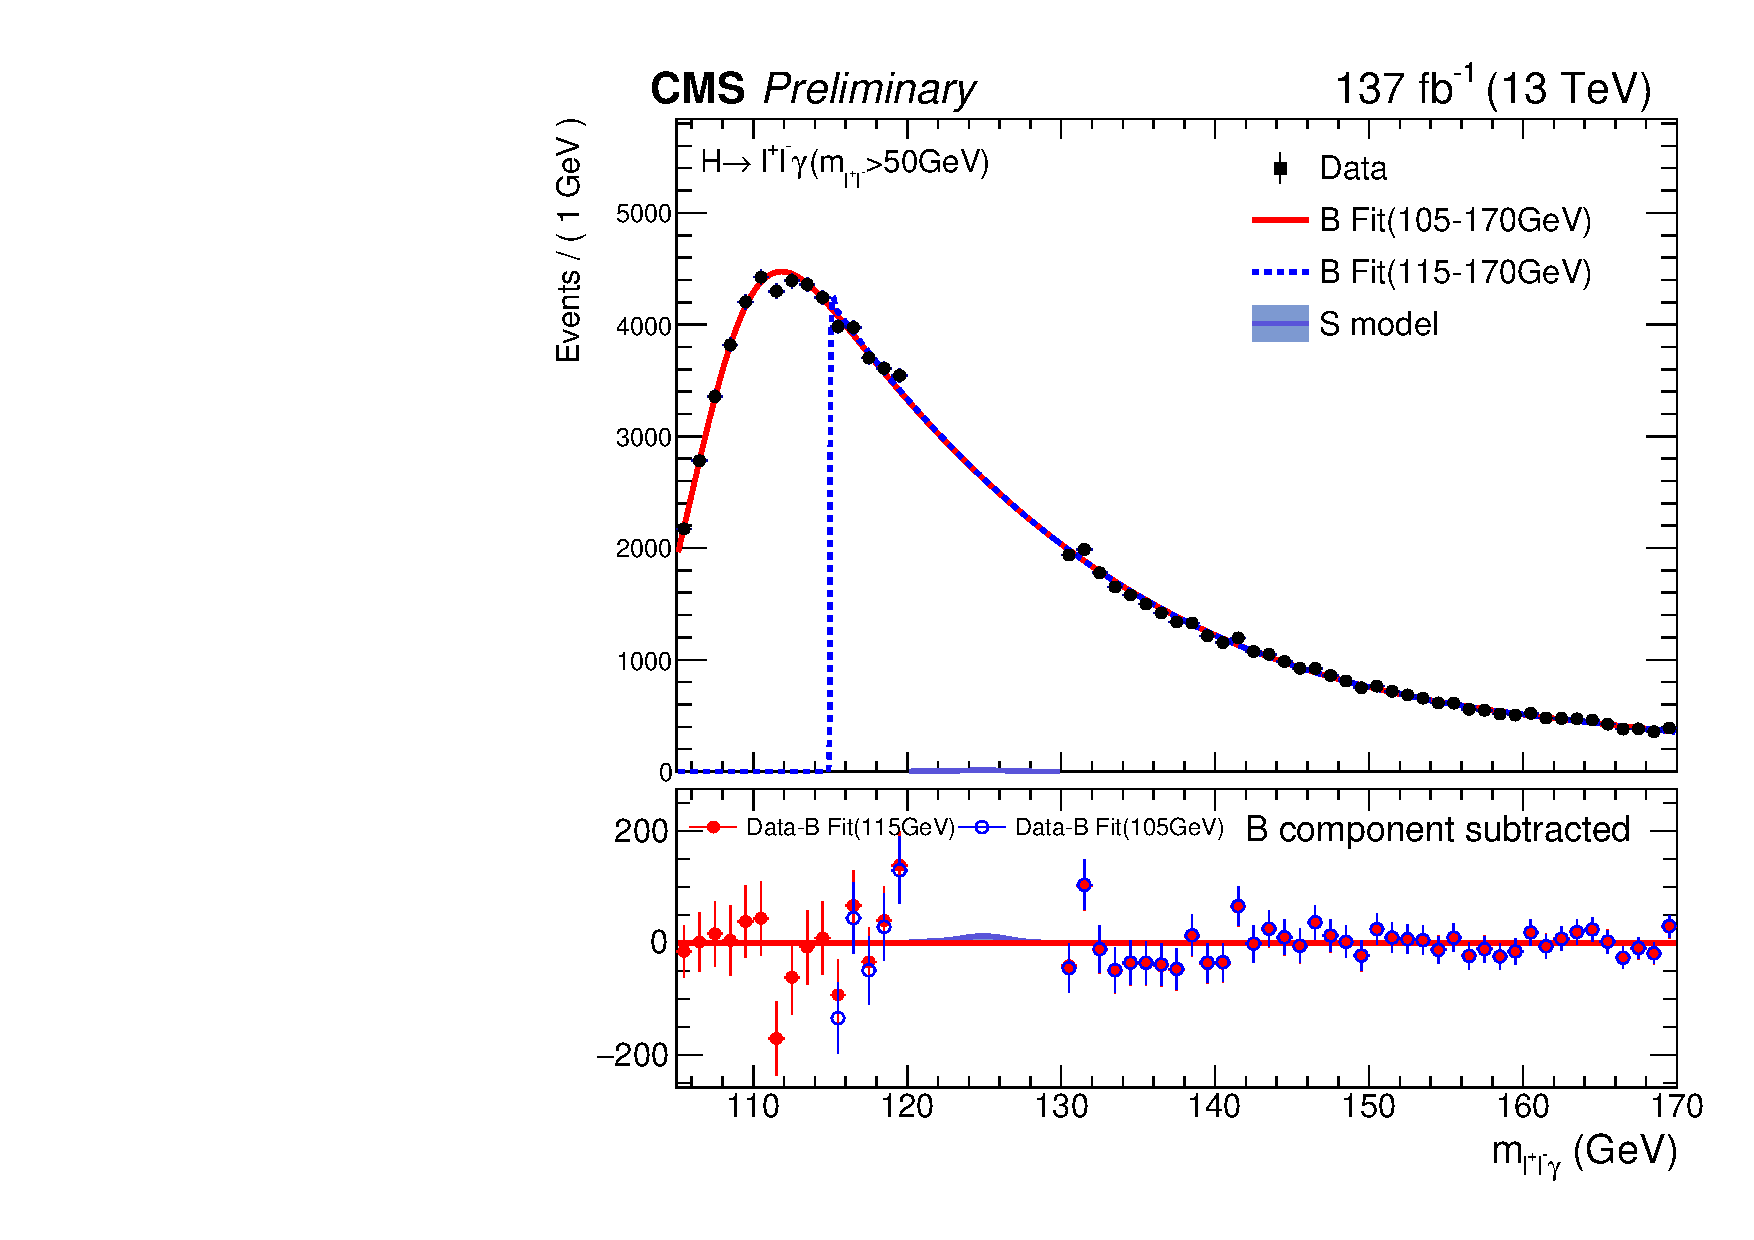
\includegraphics[width=0.27\textwidth]{fig/turnon_comparison/plot_cat4_prefit_new.pdf}\\
        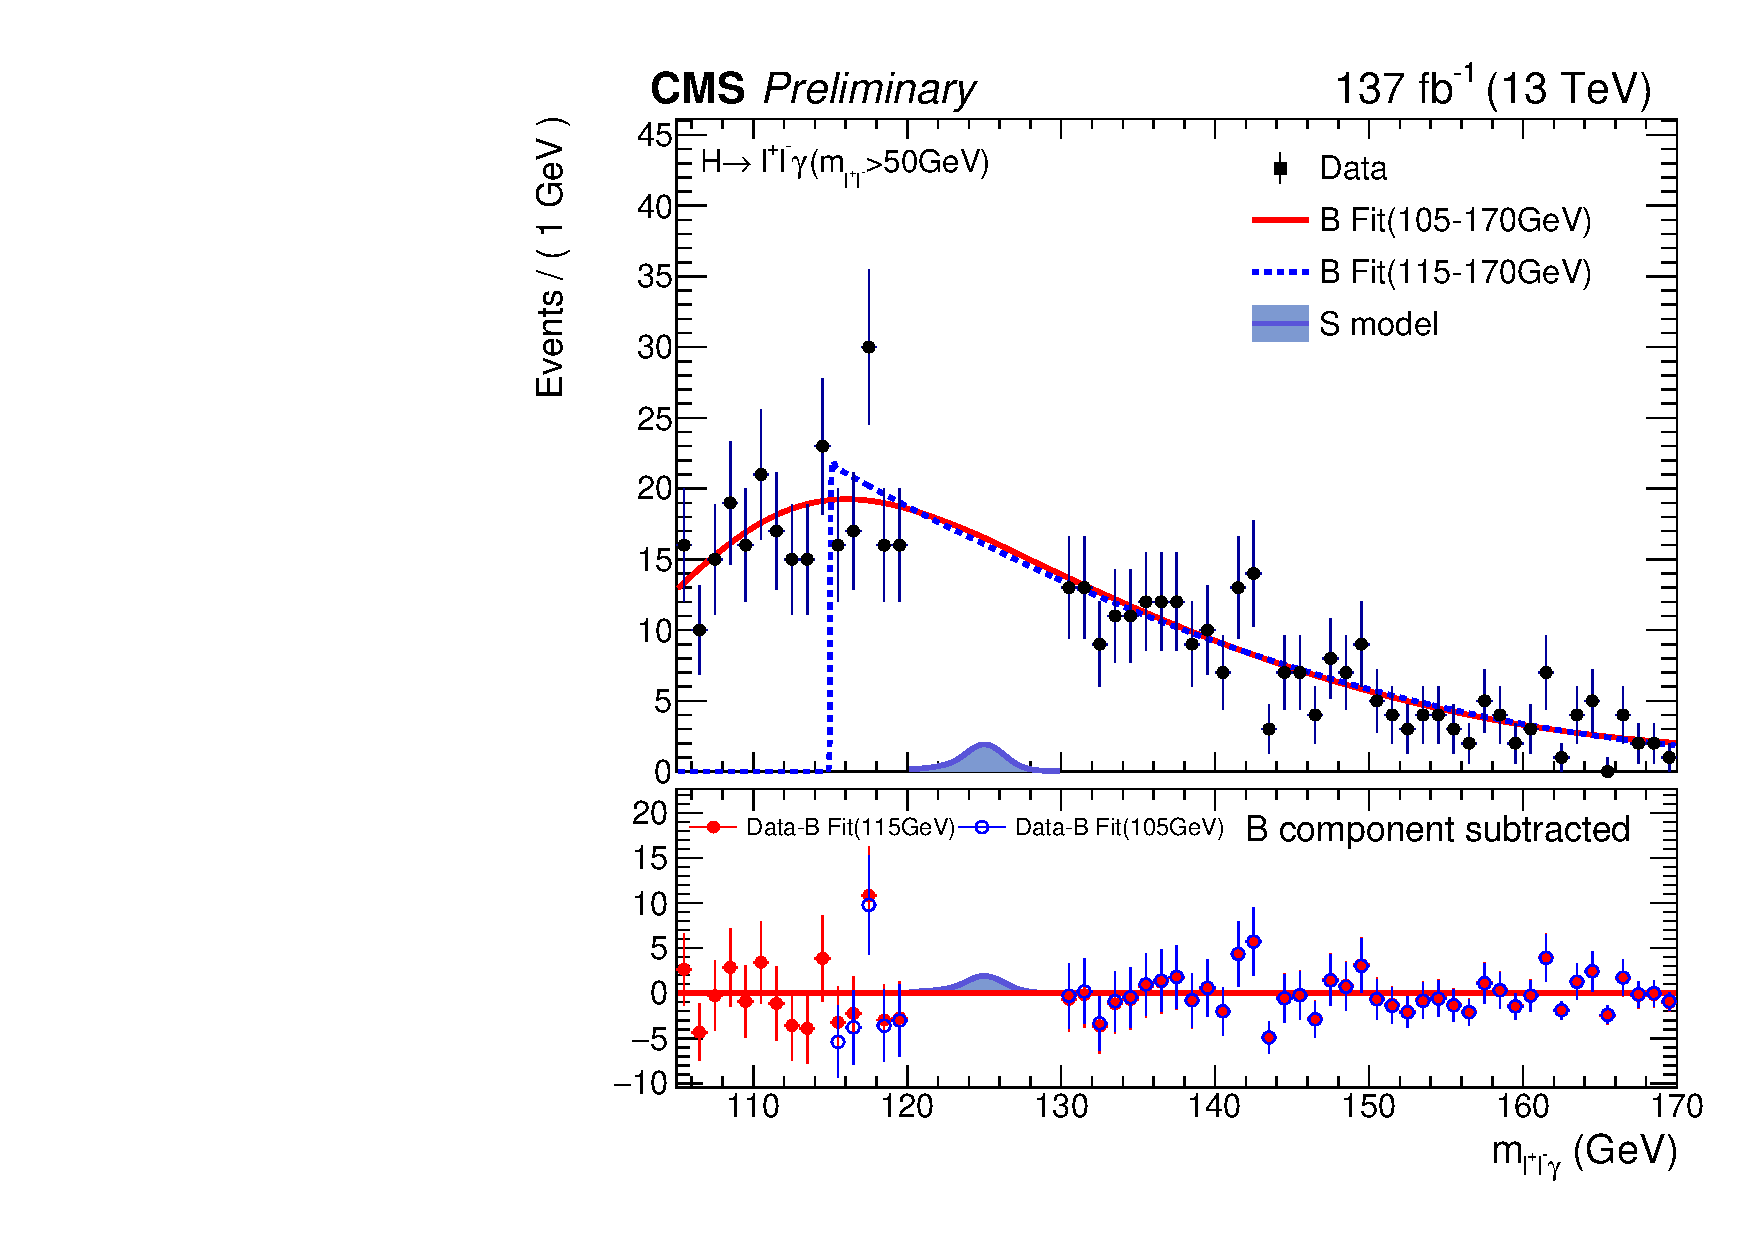
\includegraphics[width=0.27\textwidth]{fig/turnon_comparison/over_cat501_prefit_new.pdf}
        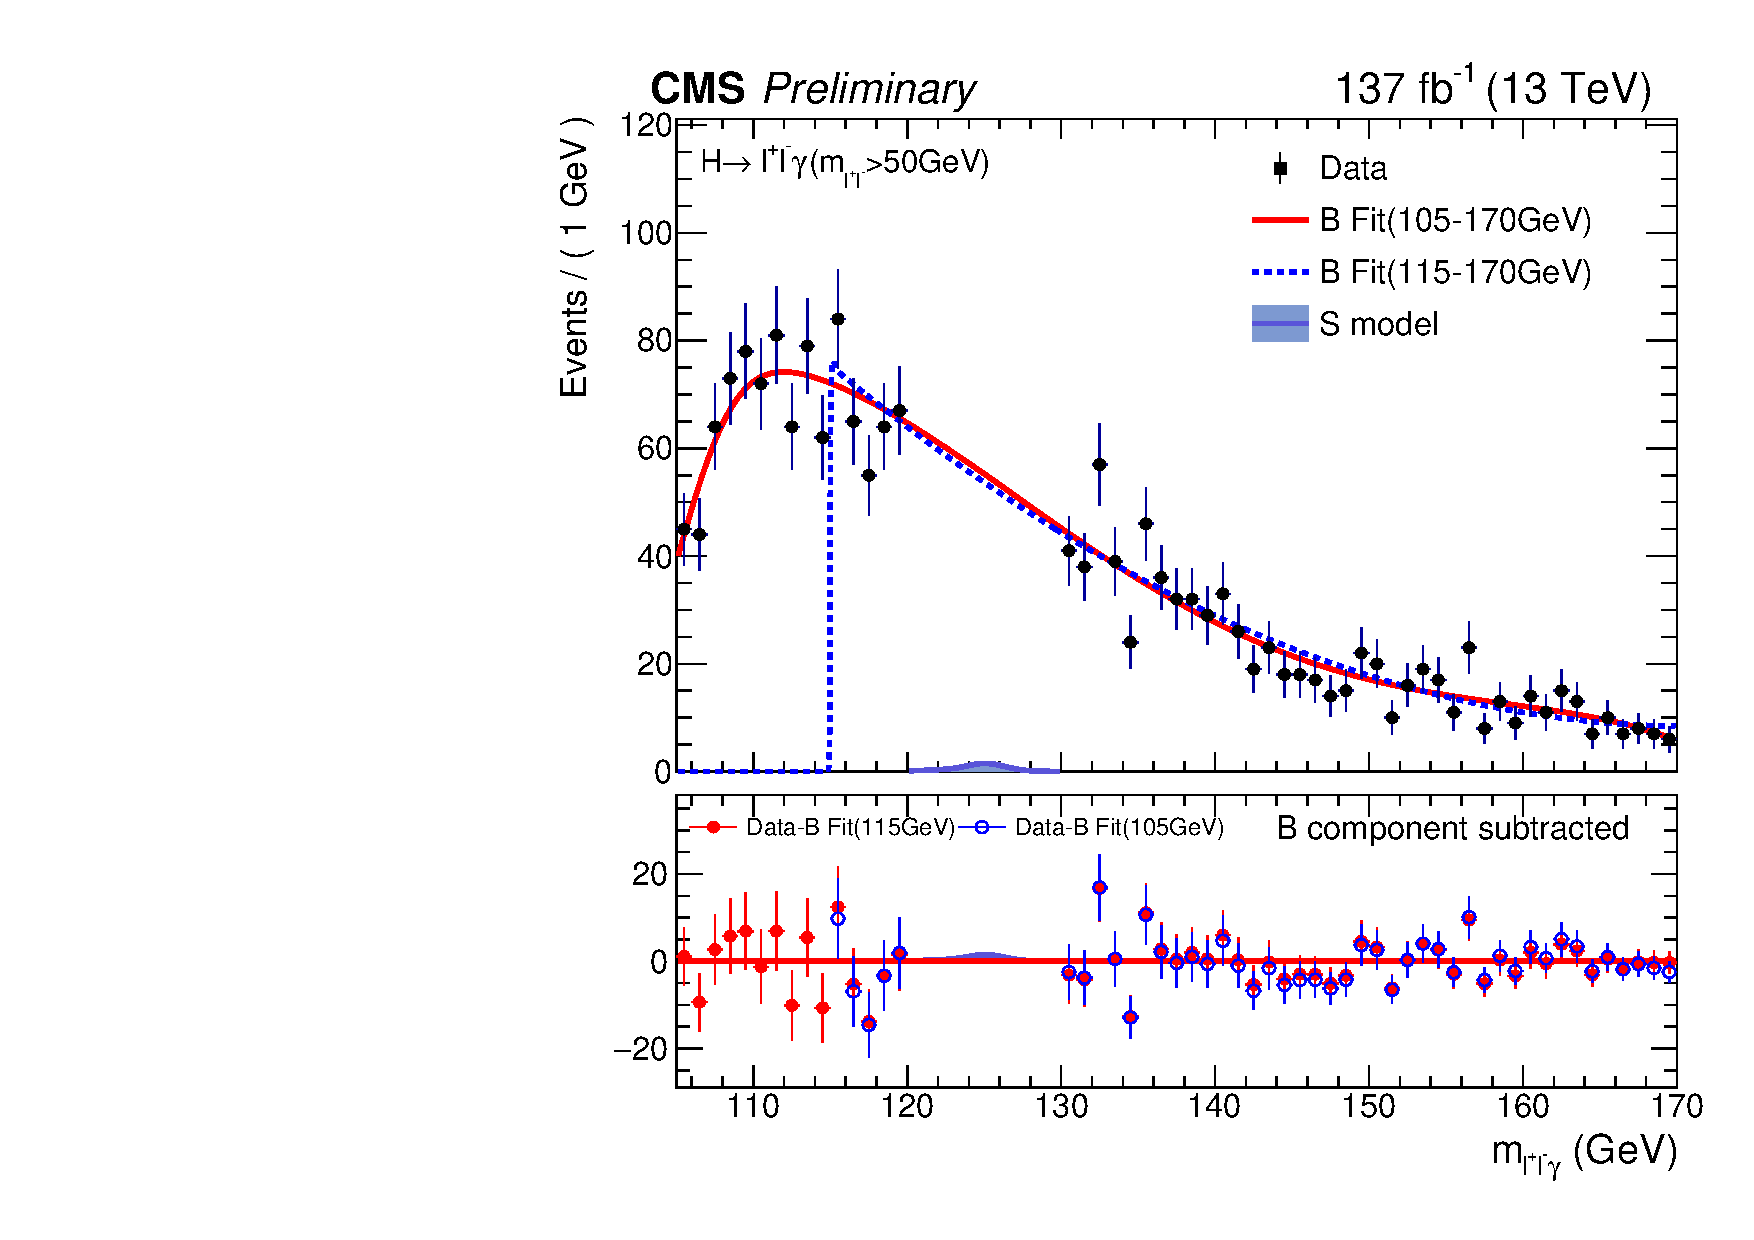
\includegraphics[width=0.27\textwidth]{fig/turnon_comparison/over_cat502_prefit_new.pdf}\\
        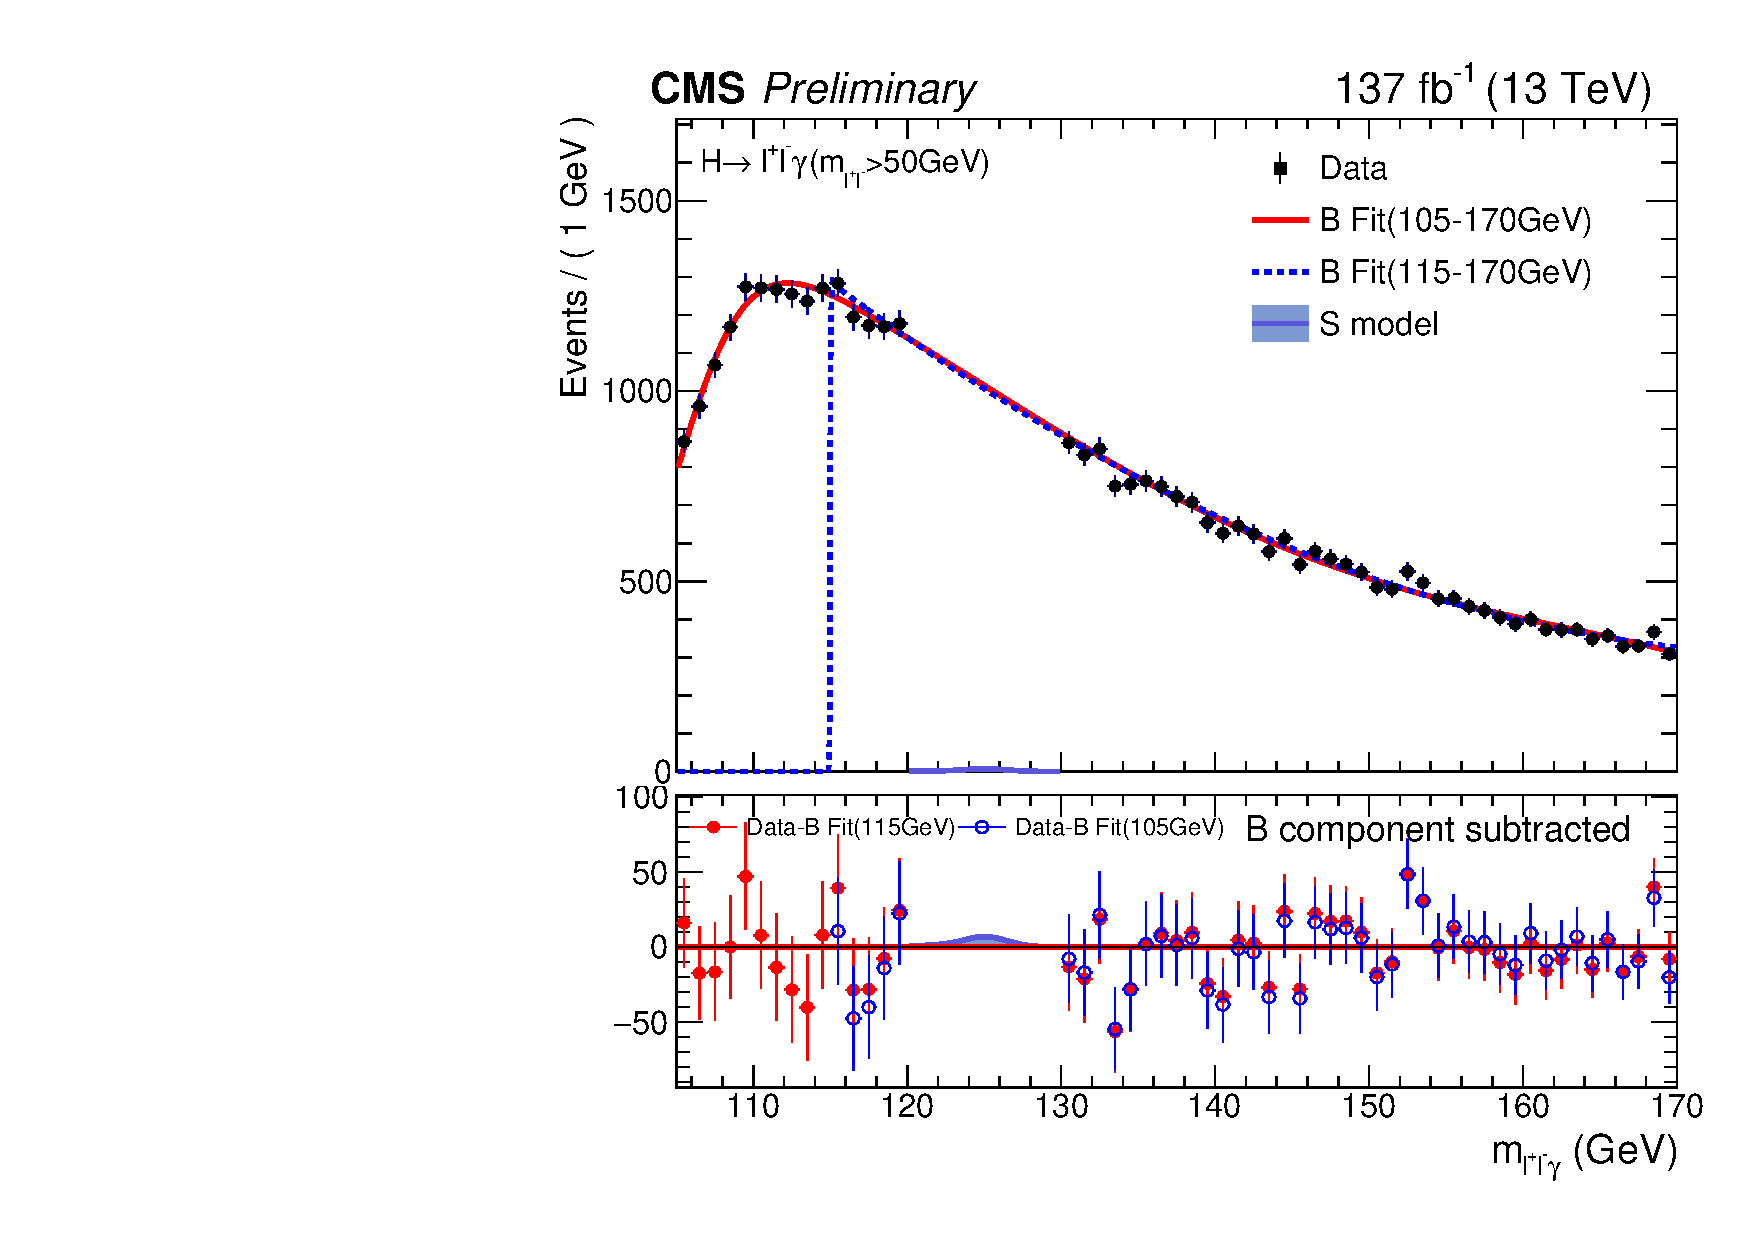
\includegraphics[width=0.27\textwidth]{fig/turnon_comparison/plot_cat503_prefit_new.pdf}
        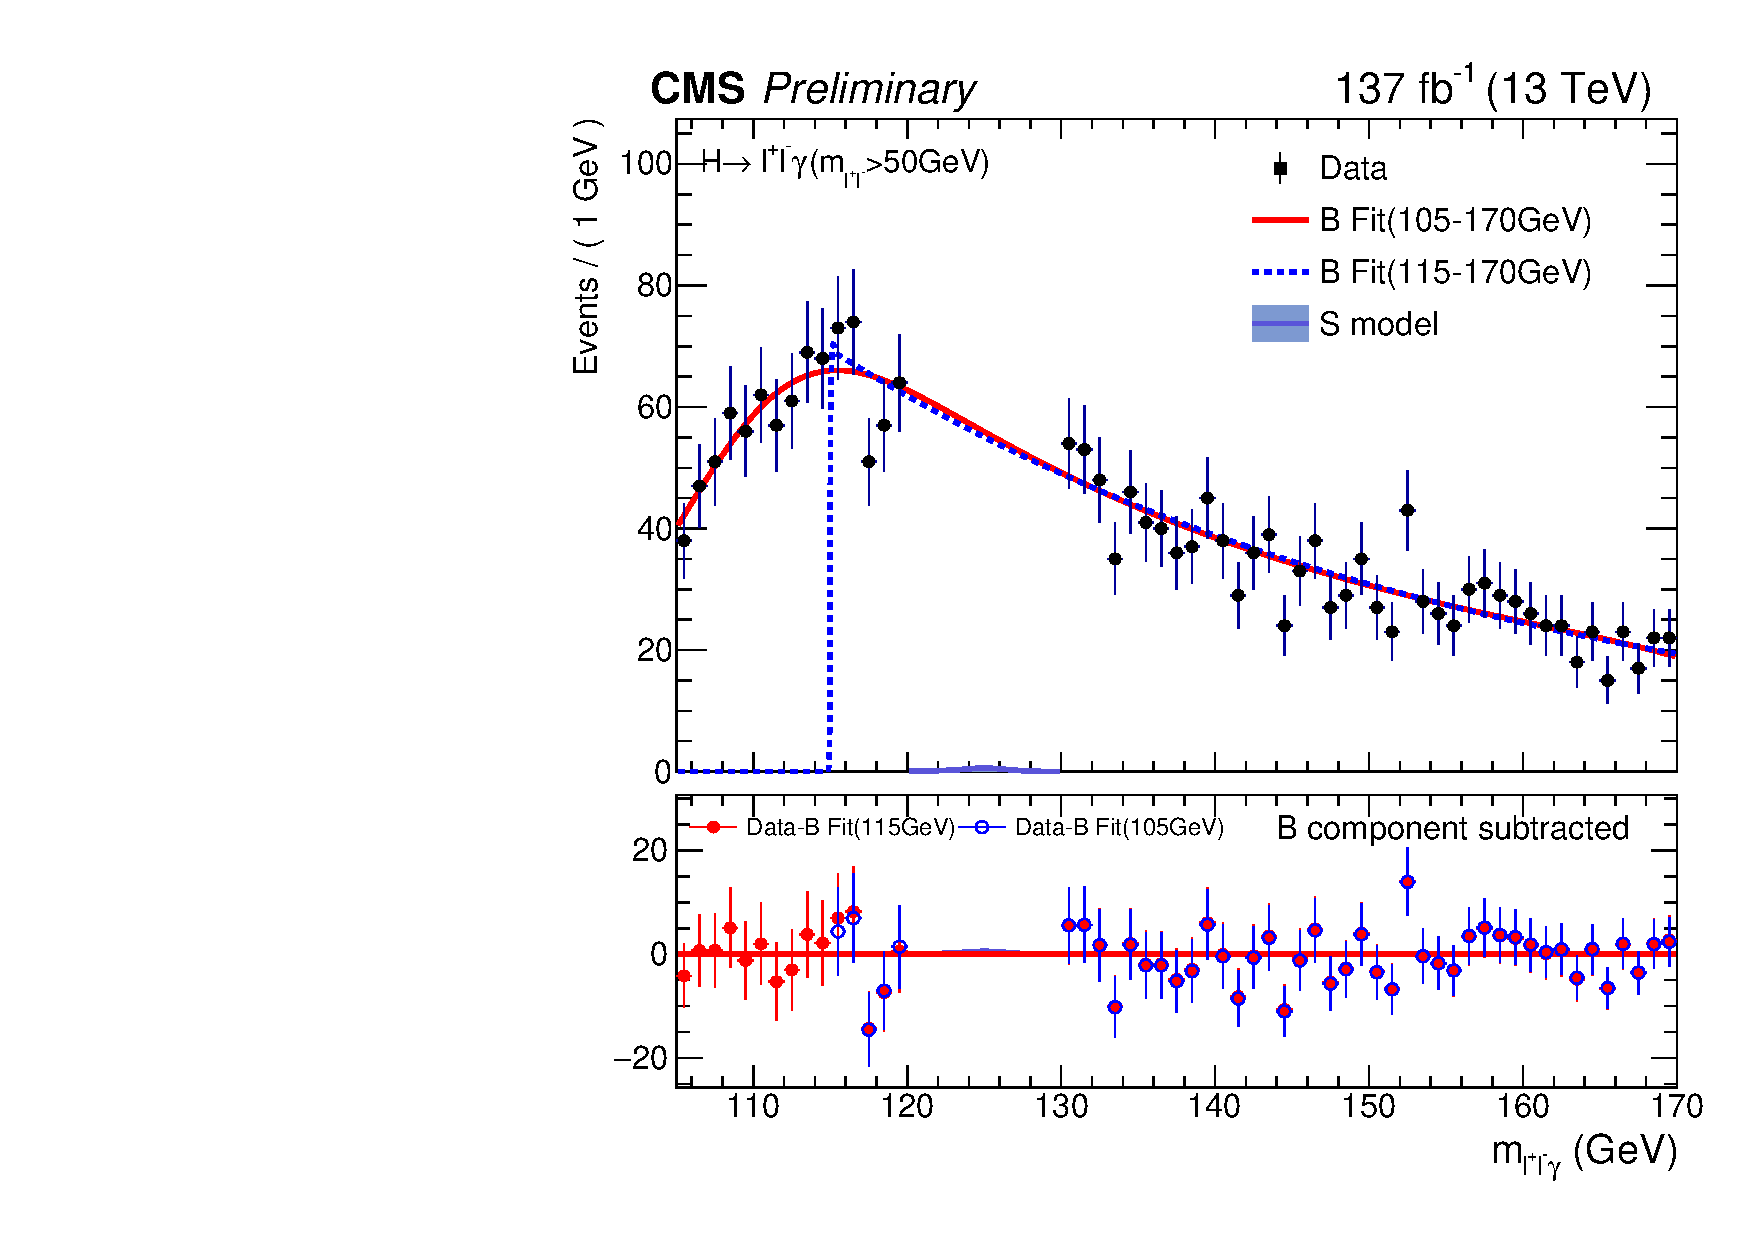
\includegraphics[width=0.27\textwidth]{fig/turnon_comparison/over_plot6789_prefit_new.pdf}
        \caption{Comparison of background fits with and without modeling the turn-on. 
        The top four plots correspond to the untagged categories, and the bottom four plots correspond to the dijet categories and lepton-tagged category.}
		\label{fig:compare_turnon_fits}
	\end{center}
\end{figure}

\subsection{Falling Spectrum Component Families}
The choice of falling spectrum component to model the background in a given category is not a priori known. For this reason, we consider several function families for the falling spectrum. 
The families considered include exponential functions, power law functions, Laurent series, and Bernstein polynomials.
These families are described in more detail below.

\begin{itemize}
	\item exponential series of order N:
	\begin{equation}
        \mathrm{Exp_{N}}(m_{\lplm\gamma}) = \sum\limits_{i=1}^{N}f_ie^{p_i\, m_{\lplm\gamma}}
	\end{equation}
	with $2N$ free parameters: $p_i < 0$ and $f_i$.
	The lowest order considered has $N=1$, i.e. one term.
	The next order has 2 exponential terms, but 3 parameters.	

	\item power law series of order N:
	\begin{equation}
        \mathrm{Pow_{N}}(m_{\lplm\gamma}) = \sum\limits_{i=1}^{N}f_im_{\lplm\gamma}^{p_i}
	\end{equation}
	with $2N$ free parameters: $p_i < 0$ and $f_i$.
	The lowest order considered has $N=1$, i.e. one term.
	
	\item Laurent series with 2, 3, 4, 5, or 6 terms, where N + 1 equals the number of free parameters:
	\begin{equation}
        \mathrm{Lau_{1}}(m_{\lplm\gamma}) = f_2m_{\lplm\gamma}^{-4}+f_3m_{\lplm\gamma}^{-5}
	\end{equation}
	\begin{equation}
        \mathrm{Lau_{2}}(m_{\lplm\gamma}) = f_1m_{\lplm\gamma}^{-3}+f_2m_{\lplm\gamma}^{-4}+f_3m_{\lplm\gamma}^{-5}
	\end{equation}
	\begin{equation}
        \mathrm{Lau_{3}}(m_{\lplm\gamma}) = f_1m_{\lplm\gamma}^{-3}+f_2m_{\lplm\gamma}^{-4}+f_3m_{\lplm\gamma}^{-5}+f_4m_{\lplm\gamma}^{-6}
	\end{equation}
	\begin{equation}
        \mathrm{Lau_{4}}(m_{\lplm\gamma}) = f_1m_{\lplm\gamma}^{-2}+f_2m_{\lplm\gamma}^{-3}+f_3m_{\lplm\gamma}^{-4}+f_4m_{\lplm\gamma}^{-5}+f_5m_{\lplm\gamma}^{-6}
	\end{equation}
	\begin{equation}
        \mathrm{Lau_{5}}(m_{\lplm\gamma}) = f_1m_{\lplm\gamma}^{-2}+f_2m_{\lplm\gamma}^{-3}+f_3m_{\lplm\gamma}^{-4}+f_4m_{\lplm\gamma}^{-5}+f_5m_{\lplm\gamma}^{-6}+f_6m_{\lplm\gamma}^{-7}
	\end{equation}
	
	\item Bernstein polynomial of order N:
    \begin{equation}
        \mathrm{Bern_{N}}(m_{\lplm\gamma}) = \sum\limits_{i=0}^{N}f_{i}b_{i,N}(m_{\lplm\gamma})
    \end{equation}
    \begin{equation}
        \mathrm{b_{i,N}}(m_{\lplm\gamma}) = \binom{N}{i}m_{\lplm\gamma}^{i}(1 - m_{\lplm\gamma}^{N-i})
    \end{equation}
    with $N$ free parameters $f_{i}$. The lowest order considered has $N=1$.
\end{itemize}

\subsection{Discrete Profiling Method}\label{sec:envelope}
In each category, there is ambiguity about which function to choose to model the background. 
In principle, the choice of function is a source of systematic uncertainty in the measurement. 
The discrete profiling method was developed as a way to assess this uncertainty in a formal way. 
In this method, the choice of function for the background fit is included as a 
discrete nuisance parameter in the full likelihood function. All reasonable families of 
functions should be considered, and a range of orders should be considered within each family. 
The set of functions profiled in a given category is referred to as an \textit{envelope}.
The exact composition of the envelope in each category
is based on a set of selection requirements that account for goodness of fit, an $\mathcal{F}$-test~\cite{Fisher:1922saa} procedure that determines the highest-order function to be included, 
and an assessment of bias and frequentist coverage. The details of this selection will be described later in this chapter.
When fitting the background, all functions in the envelope are tried, with a penalty term added to the likelihood 
to account for the number of free parameters in the fit and ensure that higher-order functions are not preferred a priori. When a measurement is made of 
a parameter of interest, such as the signal strength, the function with the smallest negative log likelihood, 
profiled as a function of the parameter of interest, is used. This profiling allows the best fit function to change for 
different values of the parameter of interest, so we can say that we carry out the fit with the full envelope of functions.  
The envelope yields a profile likelihood curve that is broader than the profile likelihood curve obtained from any individual function. 
This increase in breadth reflects the uncertainty associated with the choice of background function. 

\subsection{Envelope Selection}\label{sec:envelope_selection}
Individual functions are added to the envelope in a given category based on a series of selection requirements. In general, 
the requirements are related to three main factors: goodness of fit, $\mathcal{F}$-test results, and bias results. 
The simplest requirement is a basic goodness of fit cut. For each function considered, the chi-squared per number of degrees of freedom is calculated. This is 
then converted into a \textit{p}-value, or chi-squared probability. If the chi-squared probability is greater than 0.01, we consider 
the quality of the fit good enough for the envelope. Any function failing this requirement is thrown away, as it cannot
be considered a reasonable description of the background in data. 

The second consideration is the result of an $\mathcal{F}$-test. The $\mathcal{F}$-test is a way to compare functions within a specific family of 
falling spectrum component functions. It compares the fit of a lower-order function in the family to that of a higher-order function. 
While it is expected that the higher-order function will always provide a better fit, the question is whether the higher-order 
fit is better in a statistically significant way. If it is not significantly better, there is a motivation to stick to the lower-order function and exclude the higher-order function from the envelope. 
The details of the $\mathcal{F}$-test procedure are as follows. 
First, the lowest-order function in a given family is fit to the data in a given
category. Then, the next-highest-order function is fit to the same data. The difference between twice 
the negative log likelihood, $2\Delta NLL_{N+1} = 2(NLL_{N}-NLL_{N+1})$, of the two fits
can be used to determine whether the data better support the higher-order function. 
More specifically, $2\Delta NLL_{N+1}$ is distributed as a chi-squared function with $M$ degrees of 
freedom, where $M$ is the difference in the number of free parameters between the order $N+1$ 
function and the order $N$ function. For example, in the case of the first two orders of 
the exponential family, $M = 4-2 = 2$, and for the Bernstein polynomial family, $M=3-2=1$. 
After carrying out the fits and computing the negative log likelihoods, a \textit{p}-value is then calculated as 
\begin{equation}
\mathrm{p} = P(2\Delta NLL > 2\Delta NLL_{N+1} | \chi^{2}(M)).
\end{equation}
If this \textit{p}-value is less than 0.05, we state that the higher-order function is supported by the 
data, and the procedure is repeated for the next-highest-order function. Alternatively, if the 
\textit{p}-value is greater than 0.05, the higher-order function is assumed to be too flexible, 
and the $\mathcal{F}$-test ends, having found the highest-order function supported by the data.
In this analysis, we consider fits up to order 5 for each falling spectrum family.
In each family, we use this procedure to identify the highest-order function to include in the envelope. 
We then also include all lower-order functions within the family that pass the chi-squared goodness of fit criterion.

The final factor in selecting functions for the envelope is an assessment of bias and frequentist coverage. 
After constructing an initial envelope in a given 
category based on the chi-squared and $\mathcal{F}$-test results, an envelope bias study is performed. 
For this study, 1,000 pseudo-data sets are generated from each function contained in the envelope, which are subsequently fit with the full envelope, where 
the discrete index of the background function is allowed to float. 
In general, this means that different pseudo-data sets may be fit by different 
constituent functions within the envelope, and these functions may be different from the generating function. 
With the resulting collection of fits, we compute the bias and frequentist coverage of the signal strength $\mu$. 
For each fit, we obtain a best fit signal strength $\hat{\mu}$ and a 68\% confidence interval
($\hat{\mu}_{\mathrm{down}}$, $\hat{\mu}_{\mathrm{up}}$). We define the pull for each pseudo-data set as 
$(\hat{\mu}-\mu_{\mathrm{true}})/\sigma_{\hat{\mu}}$. 
The pull distribution is expected to be drawn from a unit Gaussian function. 
We fit the pull distribution with a Gaussian, and the best fit mean 
value is taken to be the bias. The coverage is defined as the frequency with which zero falls
within the confidence interval ($\hat{\mu}_{\mathrm{down}}$, $\hat{\mu}_{\mathrm{up}}$). It is expected to be 
near 68\%. If overcoverage is observed, this implies the uncertainty in the signal strength may 
be overly conservative. Within a few percent of 68\%, this is acceptable. If undercoverage of 
a significant amount is observed, this implies a problem with the model, and may mean that 
the individual functions are biased or that the envelope should be made more flexible. 

There are several possible outcomes of the bias studies in each 
category. One outcome is that the bias is minimal and the coverage good for all 
truth functions. In this case, we accept the composition of the envelope as good 
for the analysis. Another possible outcome is that one or more truth functions is 
associated with a large (significantly greater than 14\%) bias or low 
(significantly less than 68\%) coverage. In this case, we can consider adding 
more functions to the envelope to increase the flexibility of the model, and then 
retry the bias study using the extended envelope. 

The fits of the final chosen envelope functions in each category are shown in Figure~\ref{fig:bkgmodel_e}.
The corresponding bias and coverage results for the final envelope in each category 
are shown in Tables~\ref{tab:bias_cat1_m105-170}~through~\ref{tab:bias_cat6789_m105-170}. 
In the categories untagged 3, untagged 4, and dijet 3, it was observed that the initial functions chosen 
by the chi-squared and $\mathrm{F}$-test procedure showed large biases (greater than 20\%) and low coverages (less than 60\%) for 
certain truth functions. Therefore, the envelope was extended to include higher-order Bernstein polynomials up 
to order 5 for each of these categories. The bias tables for these categories reflect the results for the final 
extended envelope, including these added functions. 

\begin{figure}
	\begin{center}
        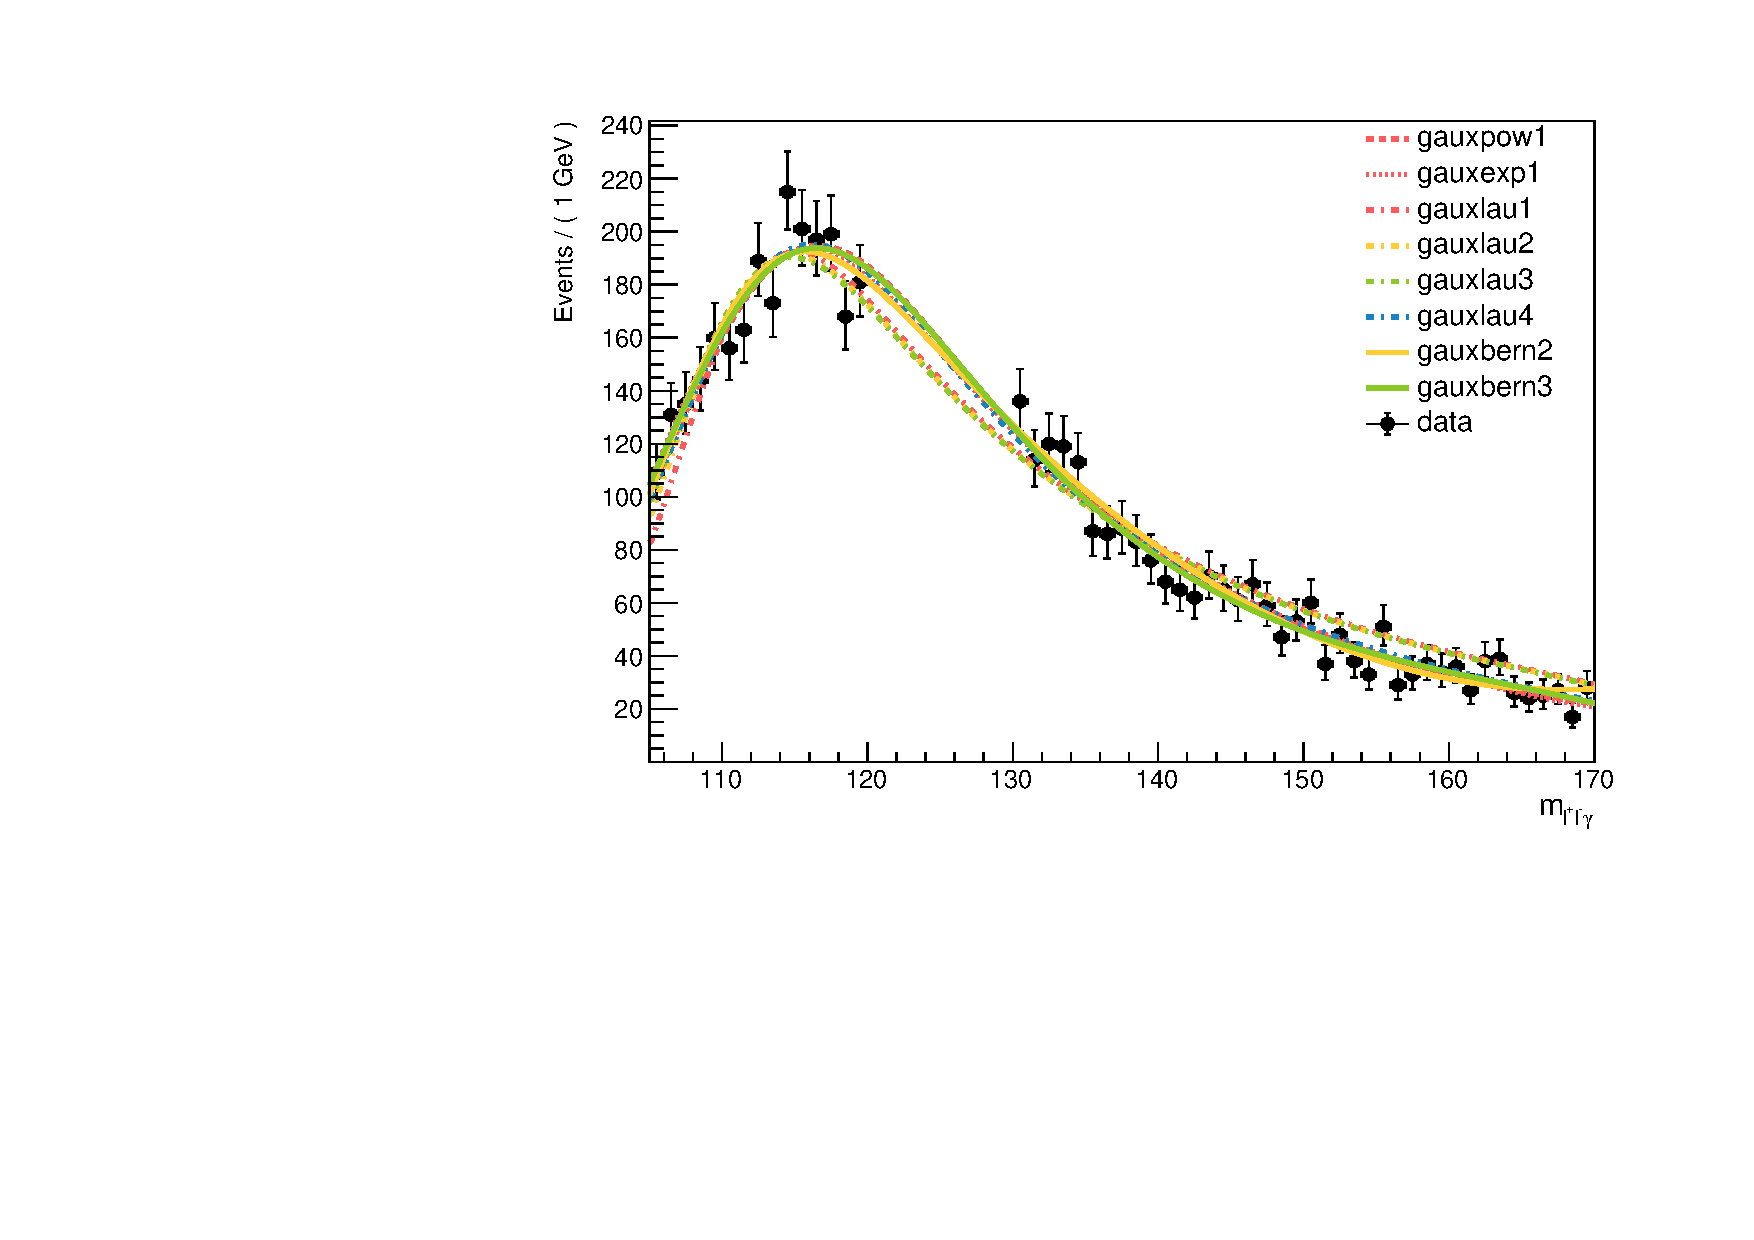
\includegraphics[width=0.4\textwidth]{fig/envelope_plots/m105_170_cat1_turn_lau.pdf}
        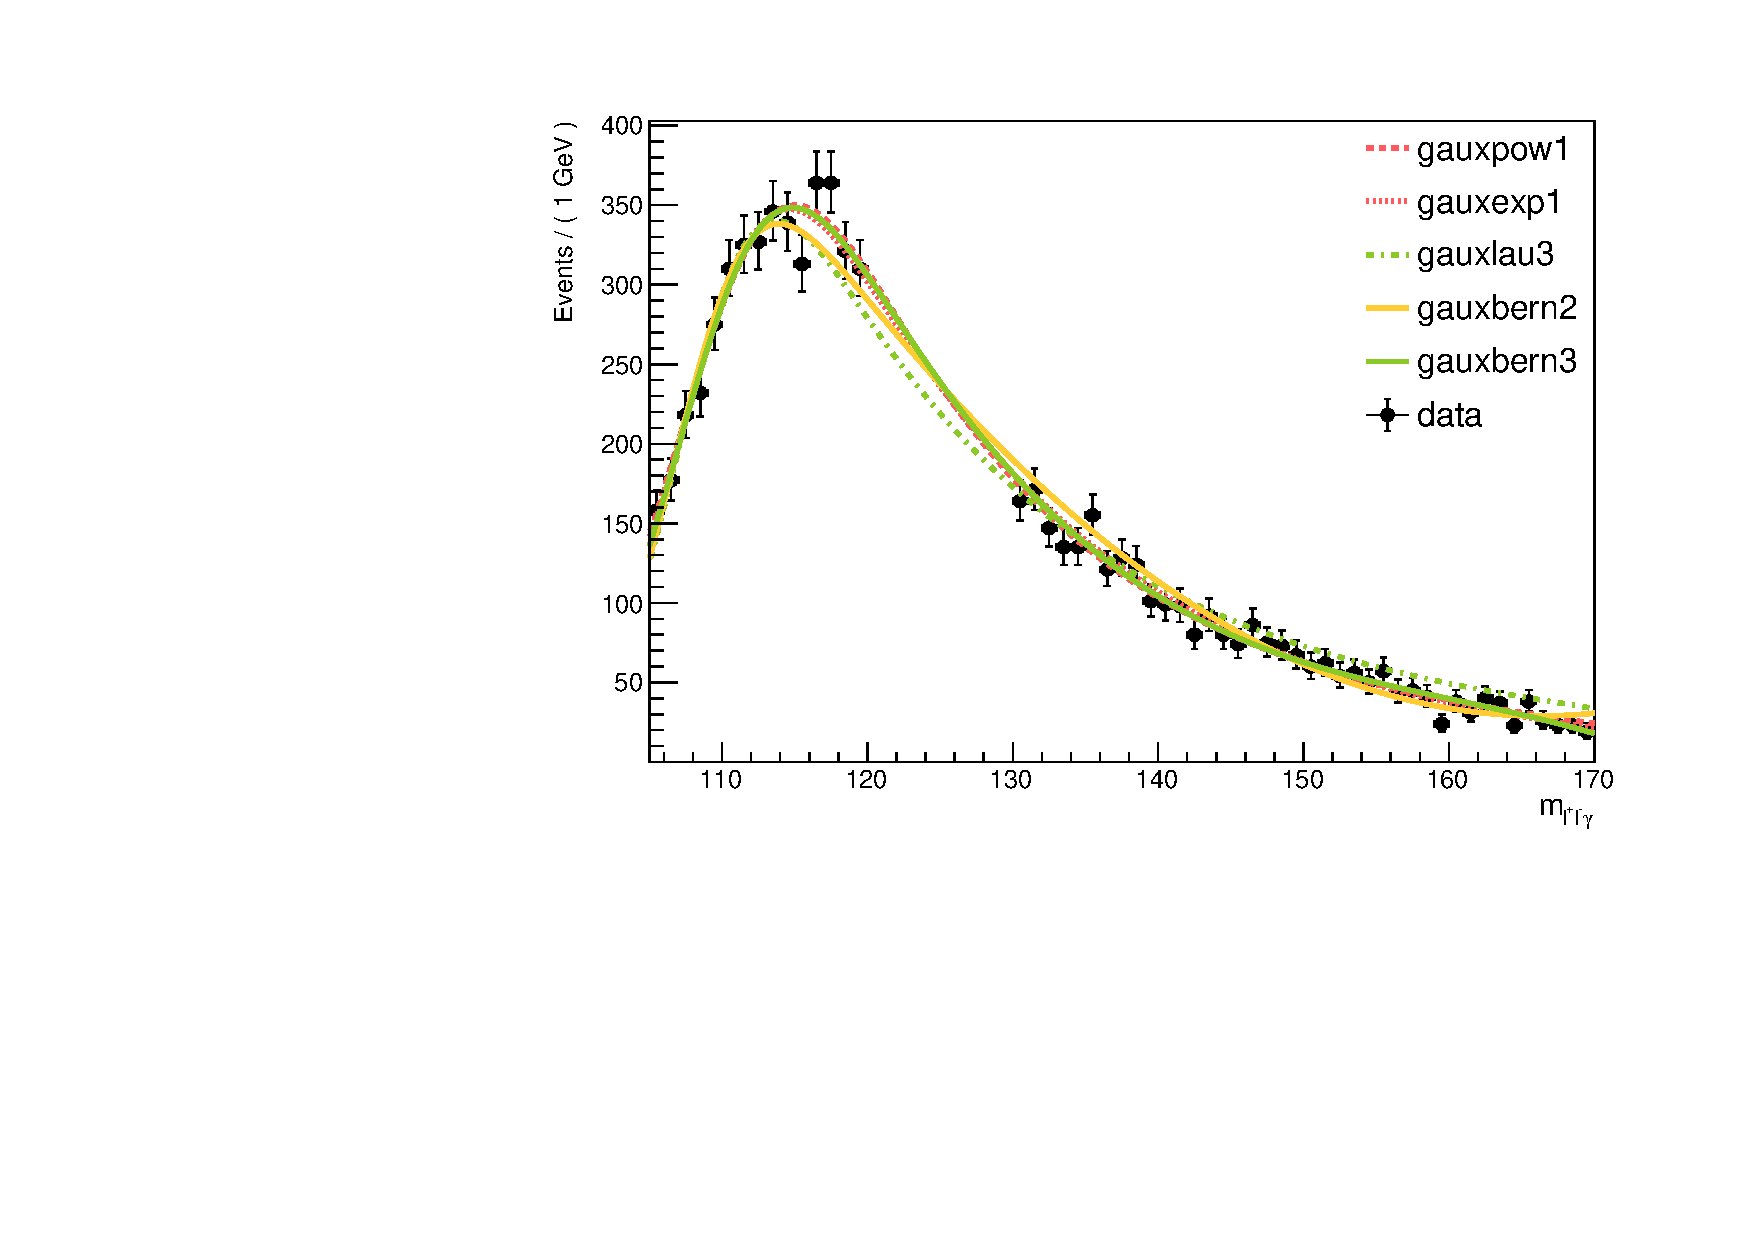
\includegraphics[width=0.4\textwidth]{fig/envelope_plots/m105_170_cat2_turn_lau.pdf}\\
        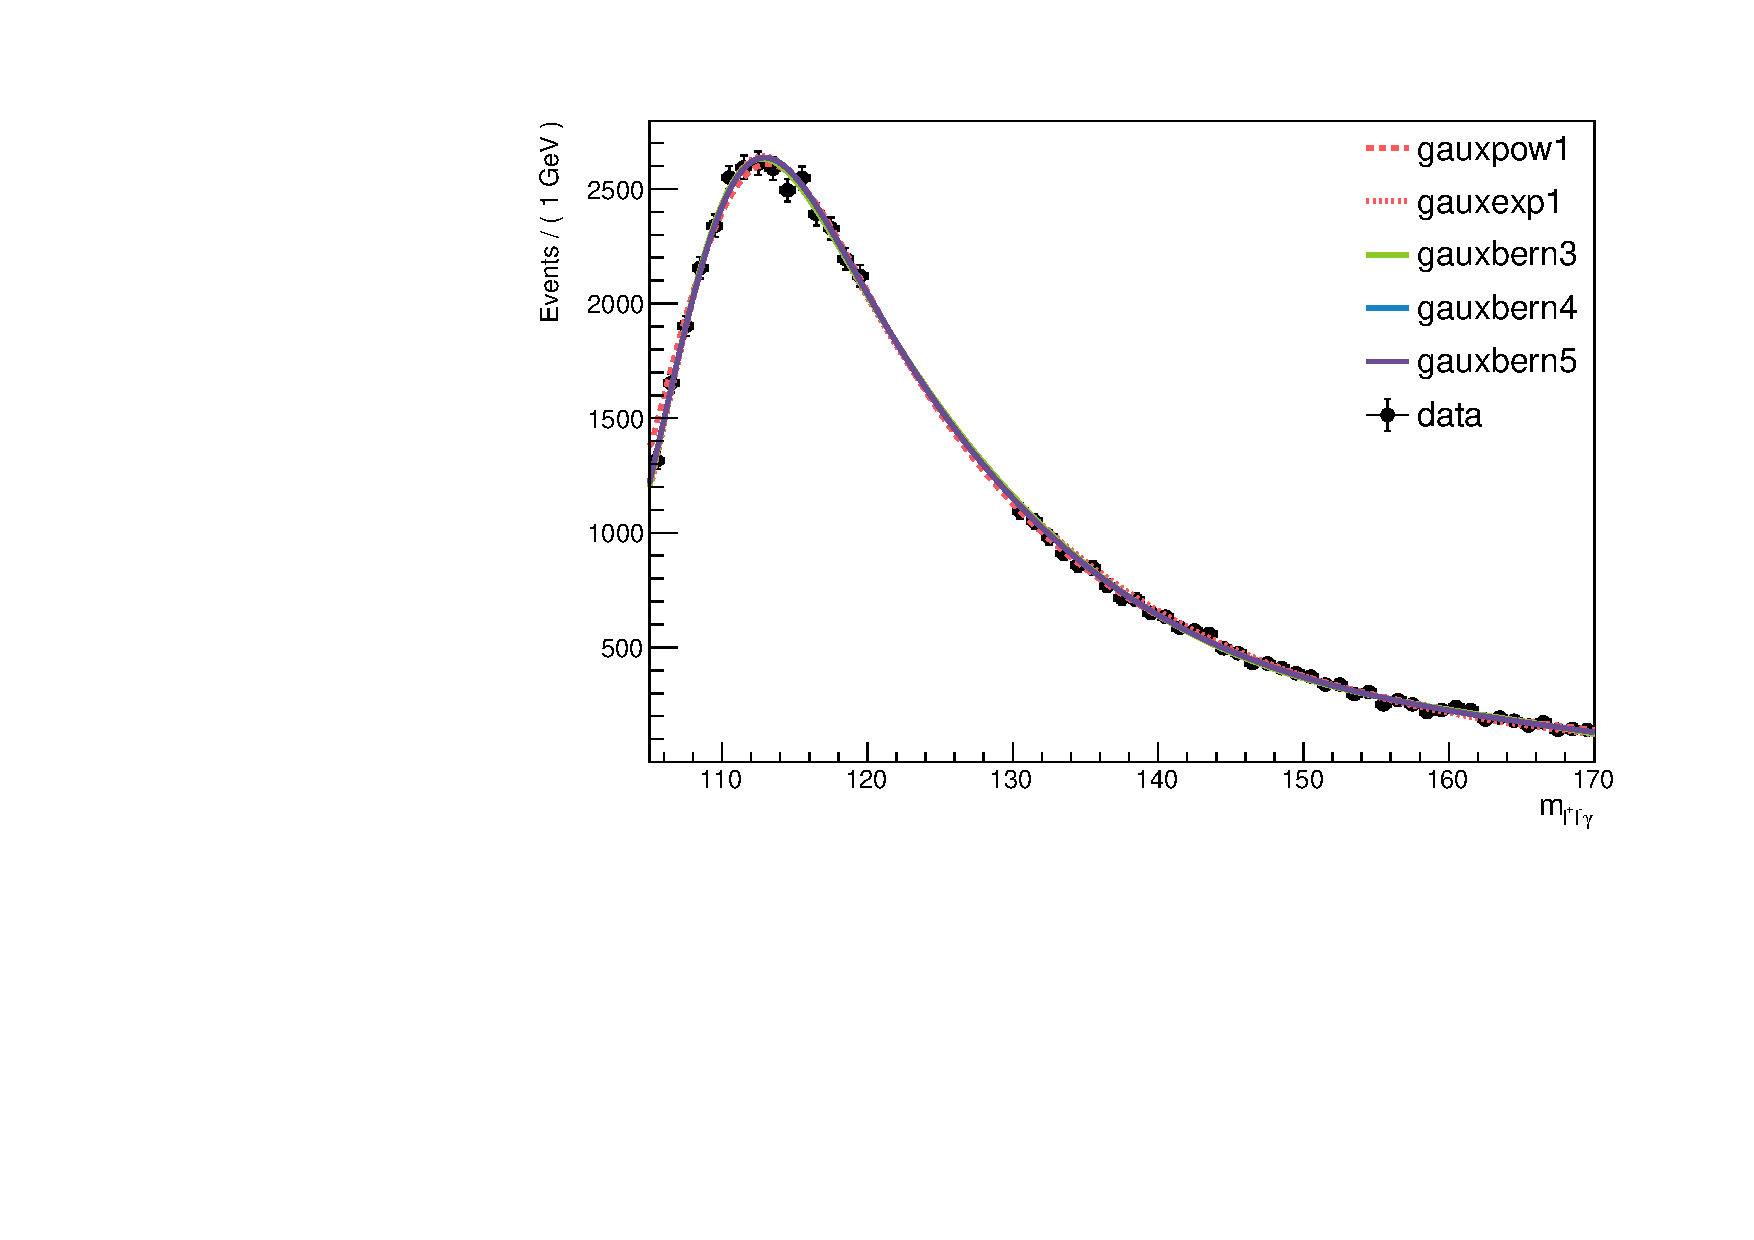
\includegraphics[width=0.4\textwidth]{fig/envelope_plots/m105_170_cat3_turn_bern5.pdf}
        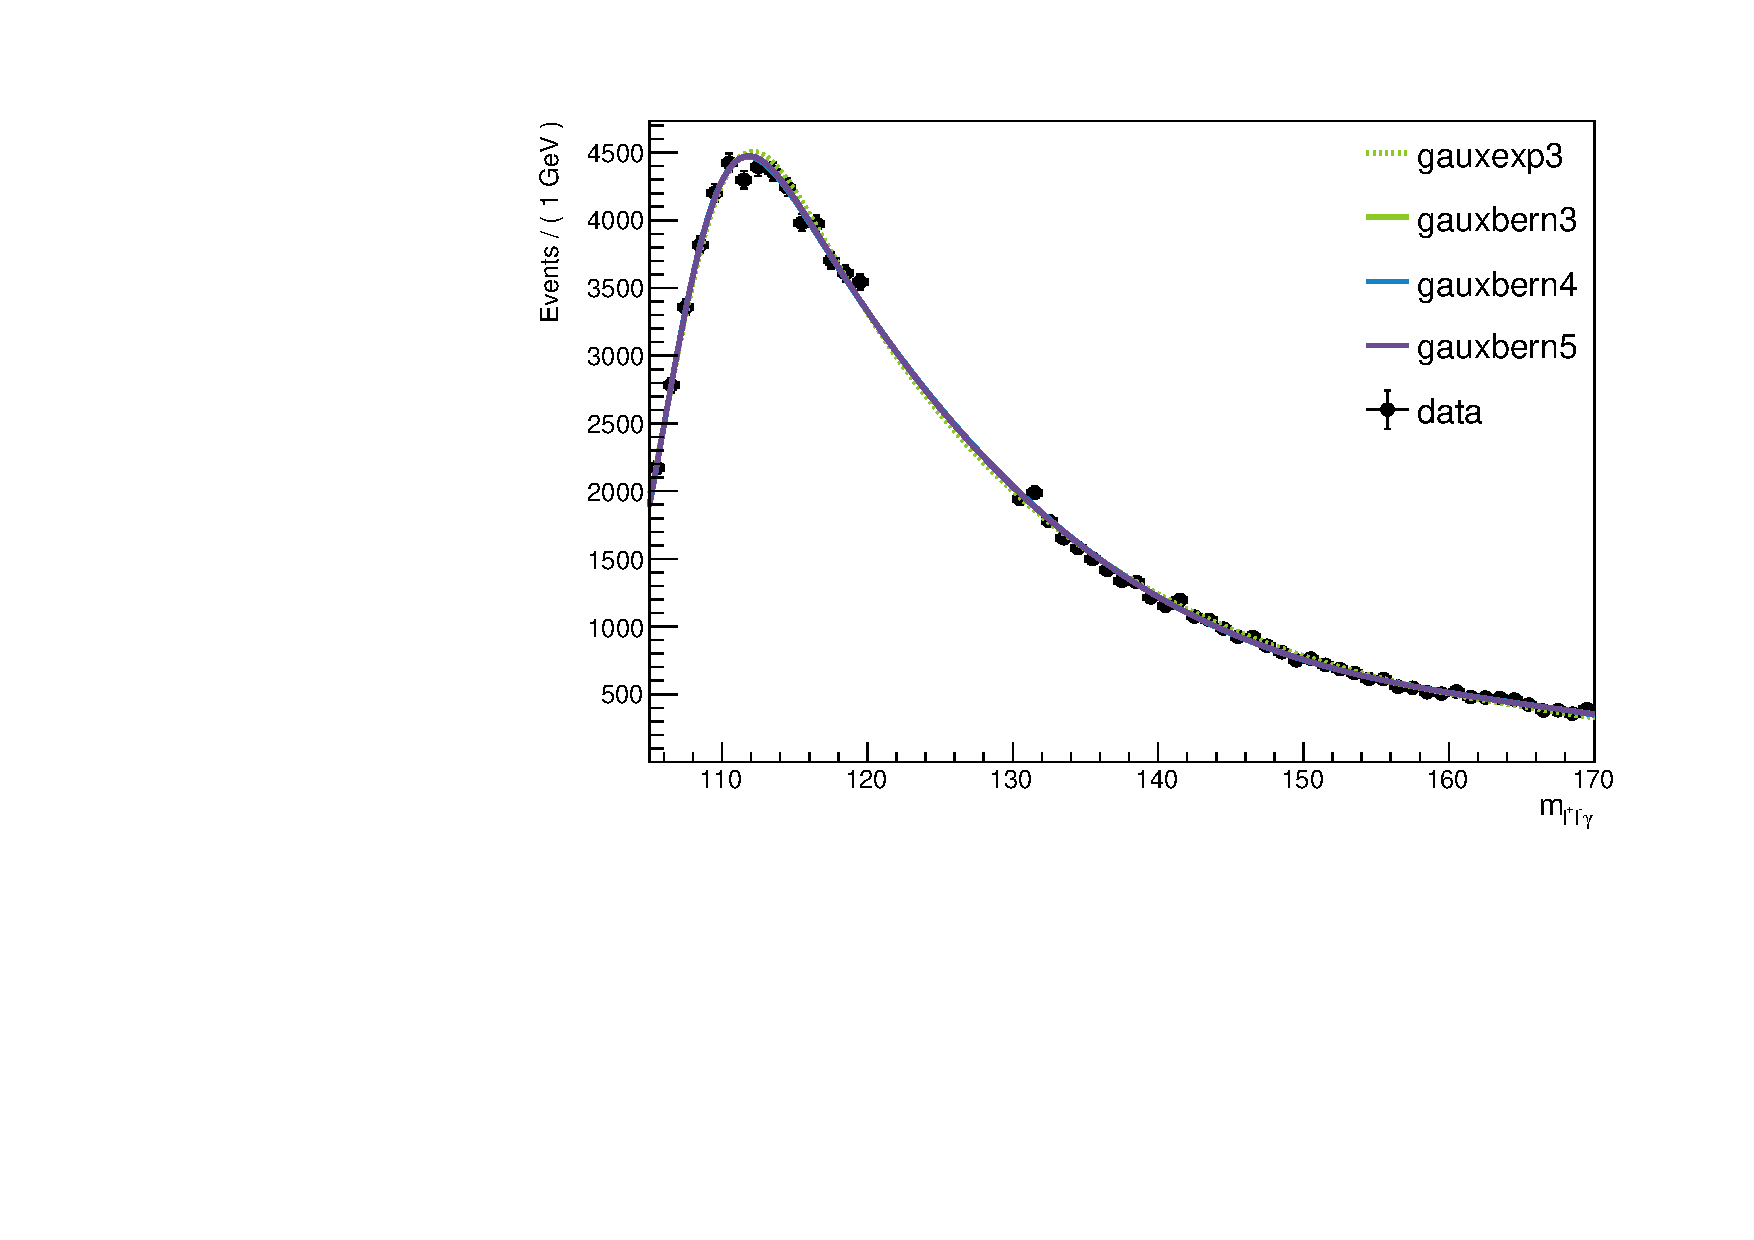
\includegraphics[width=0.4\textwidth]{fig/envelope_plots/m105_170_cat4_turn_bern5.pdf}\\
        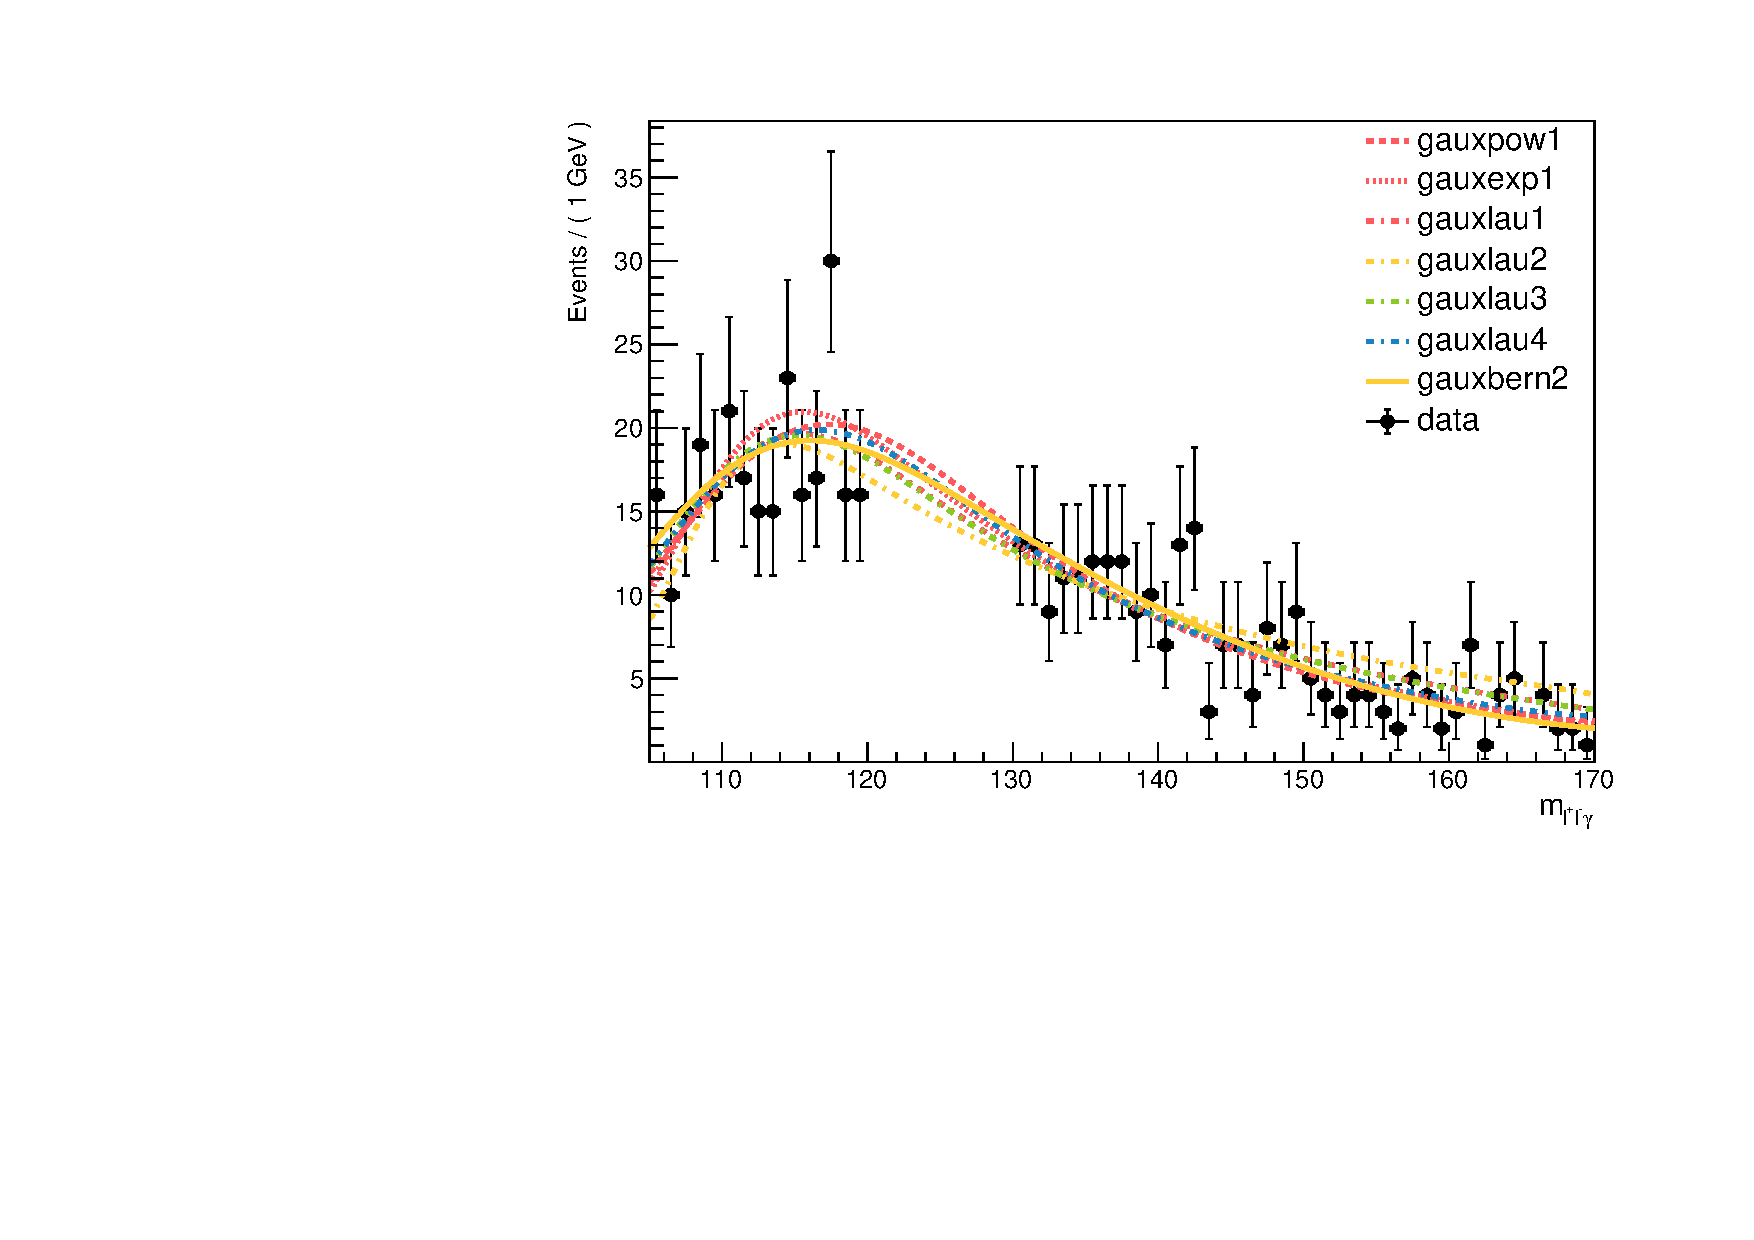
\includegraphics[width=0.4\textwidth]{fig/envelope_plots/m105_170_cat501_turn_lau.pdf}
        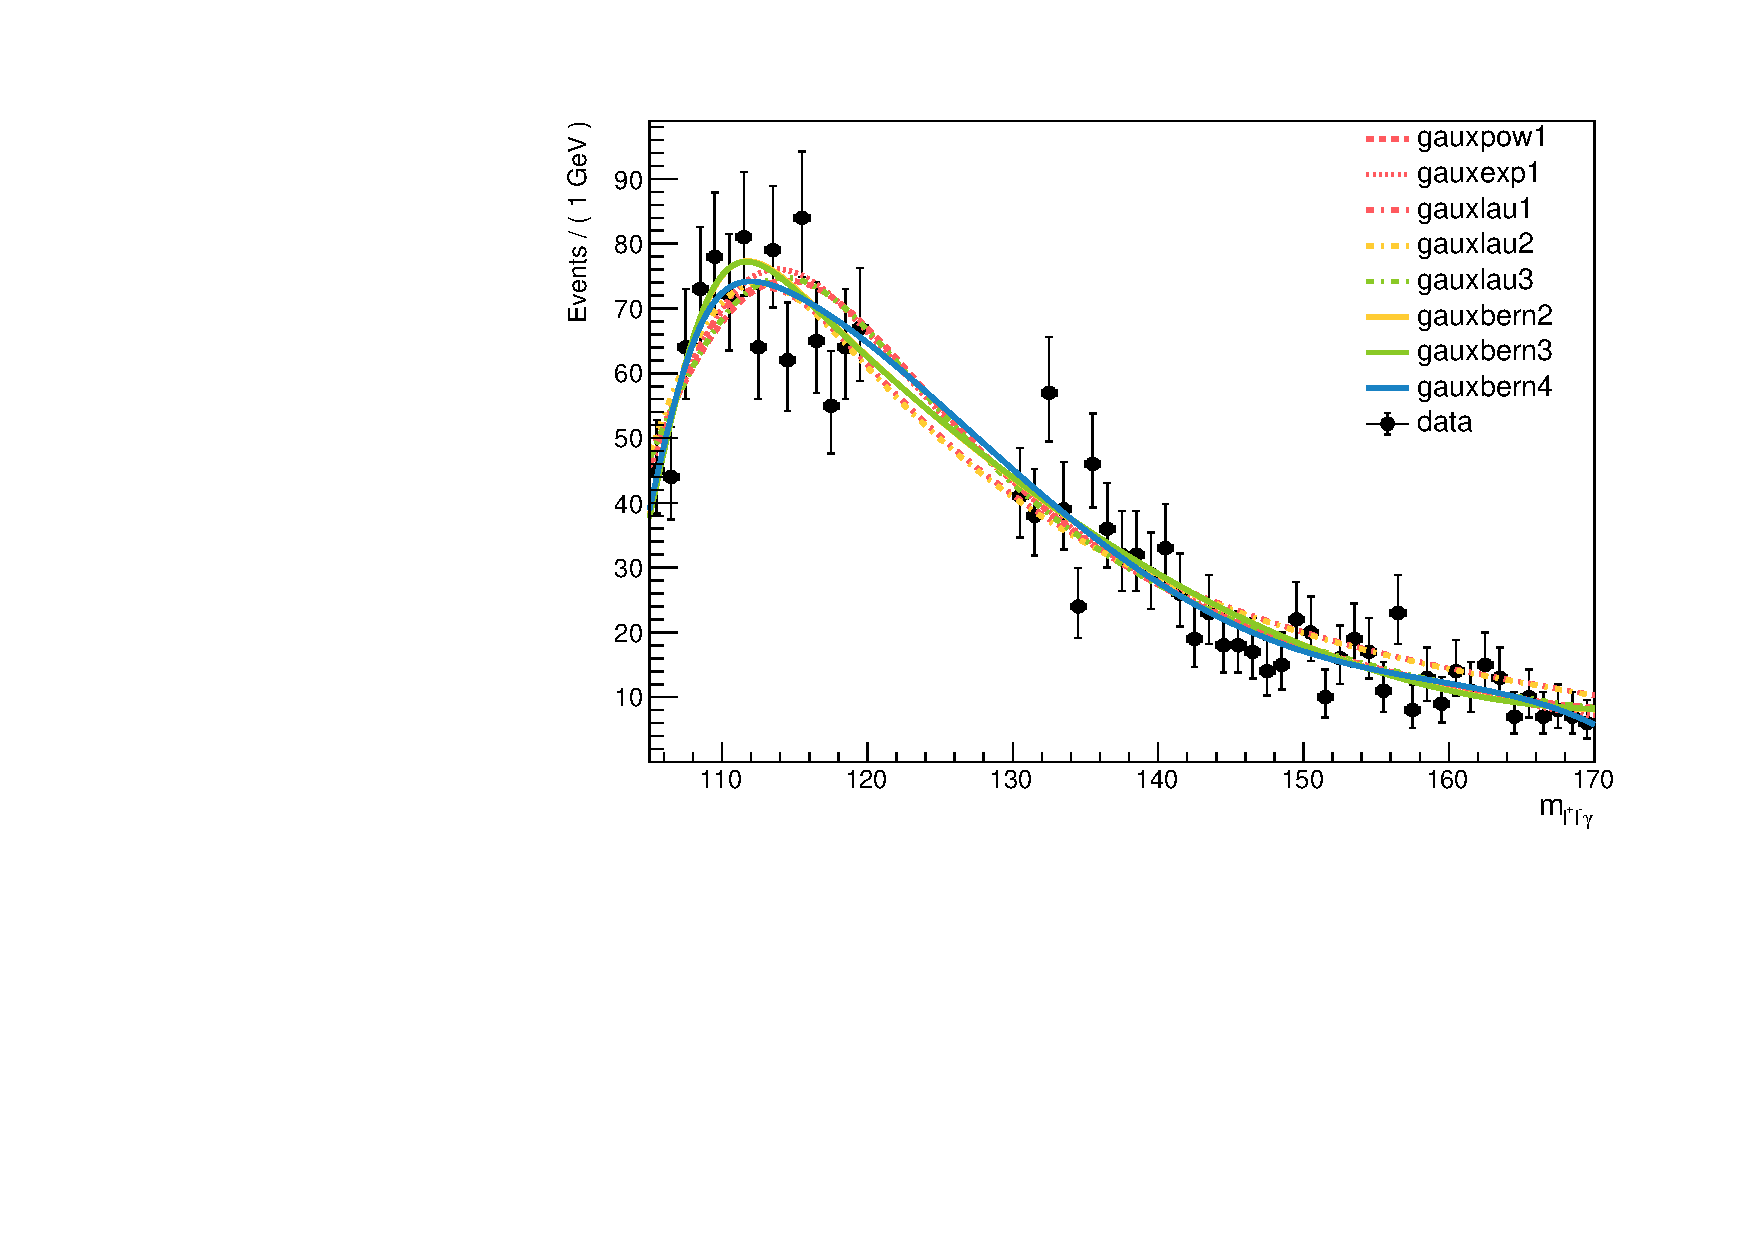
\includegraphics[width=0.4\textwidth]{fig/envelope_plots/m105_170_cat502_turn_lau.pdf}\\
        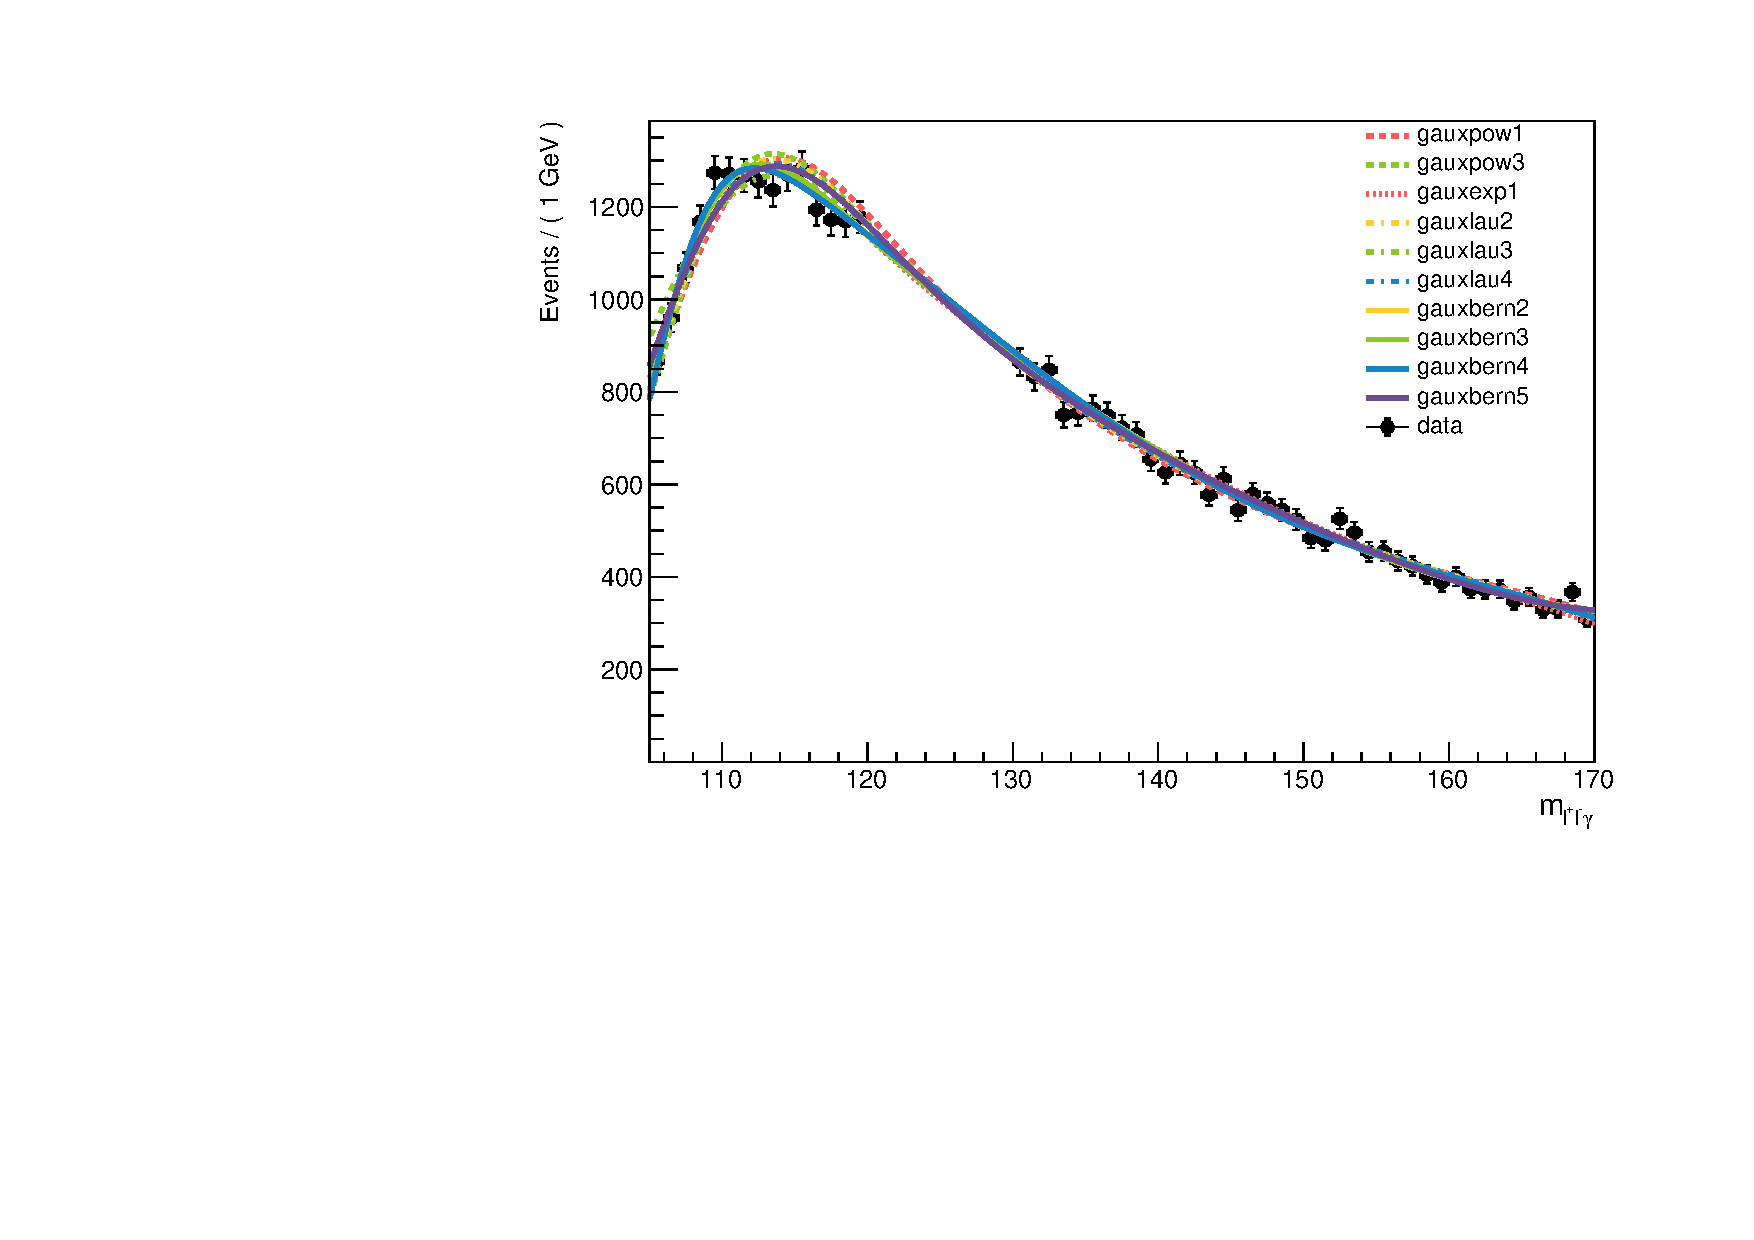
\includegraphics[width=0.4\textwidth]{fig/envelope_plots/m105_170_cat503_turn_bern5.pdf}
        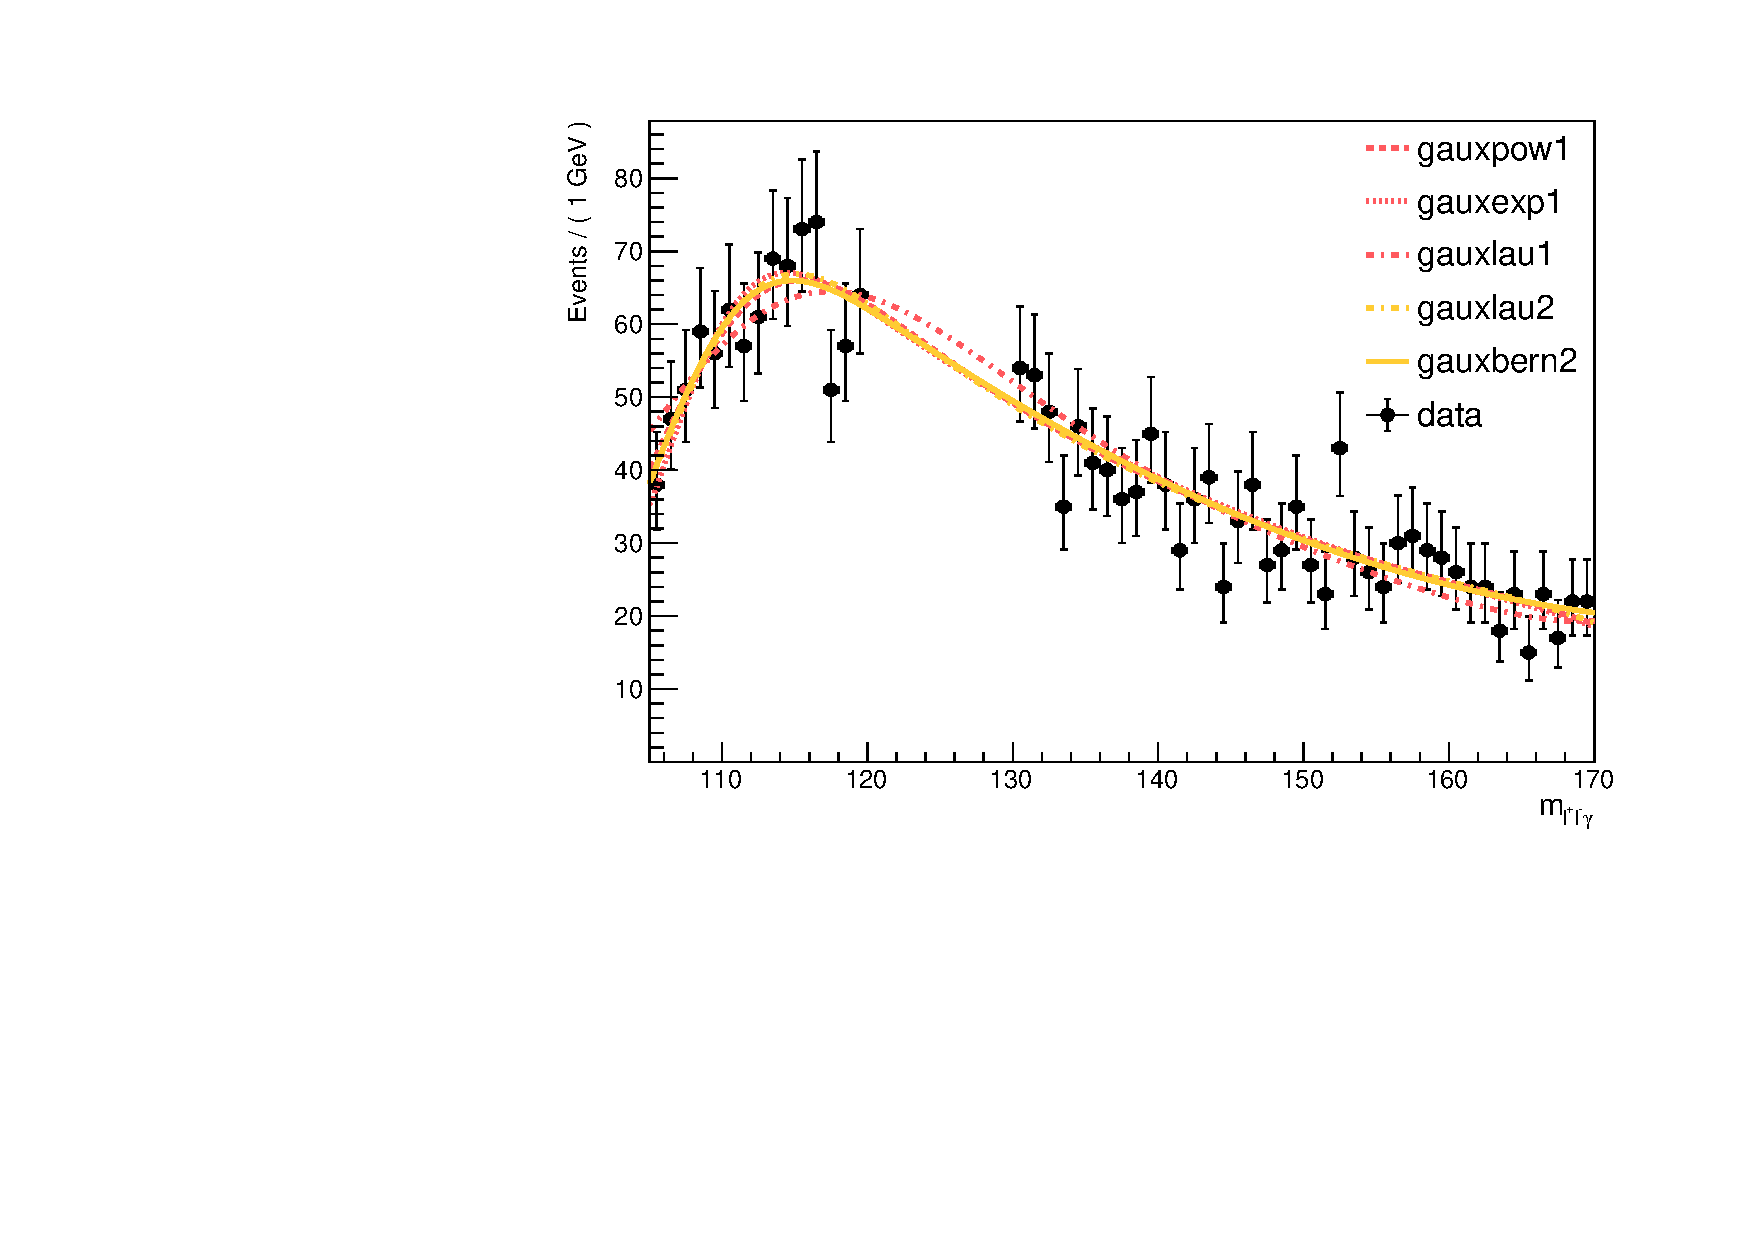
\includegraphics[width=0.4\textwidth]{fig/envelope_plots/m105_170_cat6789_turn_lau.pdf}
		\caption{Background functions selected for the envelope in each category.
        The top four plots correspond to the untagged categories, and the bottom four plots correspond to the dijet categories and lepton tag category.}
		\label{fig:bkgmodel_e}
	\end{center}
\end{figure}

\begin{table}
	\caption{Bias and coverage results for each category.}
    \footnotesize
	\centering
    \begin{subtable}{\textwidth}
	    \centering
    \begin{tabular}{|c|cccccccc|} \hline
        \textbf{Generating Function} & Exp1 & Pow1 & Lau1 & Lau2 & Lau3 & Lau4 & Bern2 & Bern3\\ \hline
        \textbf{Bias} & \tabincell{c}{-0.03\\$\pm$0.03}& \tabincell{c}{0.02\\$\pm$0.04}& \tabincell{c}{0.02\\$\pm$0.04}& \tabincell{c}{0.06\\$\pm$0.04}& \tabincell{c}{0.04\\$\pm$0.04}& \tabincell{c}{-0.09\\$\pm$0.04} &\tabincell{c}{-0.07\\$\pm$0.03} &\tabincell{c}{0.00\\$\pm$0.04}\\ 
        \textbf{Coverage} & 0.68 & 0.66 & 0.71 & 0.68 & 0.71 & 0.68 & 0.65 & 0.70\\ \hline
    \end{tabular}
    \caption{Untagged 1 bias and coverage results from the final envelope bias study.}
    \label{tab:bias_cat1_m105-170}
    \end{subtable}
    \vspace*{0.25 cm}
    \begin{subtable}{\textwidth}
        \footnotesize
        \centering
        \begin{tabular}{|c|ccccc|} \hline
            \textbf{Generating Function} &Exp1 &Pow1 &Lau3 &Bern2 &Bern3\\ \hline
            \textbf{Bias} &\tabincell{c}{-0.10\\$\pm$0.04}&\tabincell{c}{-0.09\\$\pm$0.05} &\tabincell{c}{-0.27\\$\pm$0.04}& \tabincell{c}{-0.07\\$\pm$0.03} & \tabincell{c}{0.07\\$\pm$0.04}\\ 
            \textbf{Coverage} & 0.67 & 0.66 & 0.67 & 0.67 & 0.65\\ \hline
        \end{tabular}
        \caption{Untagged 2 bias and coverage results from the final envelope bias study.}
        \label{tab:bias_cat2_m105-170}
    \end{subtable}
    \vspace*{0.25 cm}
    \begin{subtable}{\textwidth}
        \footnotesize
        \centering
        \begin{tabular}{|c|ccccc|} \hline
            \textbf{Generating Function} &Exp1 &Pow1 &Bern3&Bern4&Bern5\\ \hline
            \textbf{Bias} &\tabincell{c}{-0.05\\$\pm$0.04}&\tabincell{c}{-0.11\\$\pm$0.03}&\tabincell{c}{0.03\\$\pm$0.04}&\tabincell{c}{-0.02\\$\pm$0.03}&\tabincell{c}{0.27\\$\pm$0.04}\\ 
            \textbf{Coverage} & 0.67&0.67 & 0.70 &0.67 & 0.66\\ \hline
        \end{tabular}
        \caption{Untagged 3 bias and coverage results from the final envelope bias study.}
        \label{tab:bias_cat3_m105-170}
    \end{subtable}
    \vspace*{0.25 cm}
    \begin{subtable}{\textwidth}
        \footnotesize
        \centering
        \begin{tabular}{|c|cccc|} \hline
            \textbf{Generating Function} &Exp3 &Bern3 &Bern4 &Bern5\\ \hline
            \textbf{Bias} &\tabincell{c}{-0.08\\$\pm$0.03} &\tabincell{c}{0.07\\$\pm$0.03} &\tabincell{c}{0.16\\$\pm$0.03} &\tabincell{c}{0.10\\$\pm$0.03}\\ 
            \textbf{Coverage} & 0.68 & 0.67 & 0.67 & 0.68\\ \hline
        \end{tabular}
        \caption{Untagged 4 bias and coverage results from the final envelope bias study.}
        \label{tab:bias_cat4_m105-170}
    \end{subtable}
    \vspace*{0.25 cm}
\begin{subtable}{\textwidth}
    \footnotesize
    \centering
    \begin{tabular}{|c|ccccccc|} \hline
        \textbf{Generating Function} &Exp1 &Pow1 &Lau1 &Lau2 &Lau3 &Lau4 &Bern2\\ \hline
        \textbf{Bias} &\tabincell{c}{0.03\\$\pm$0.03} &\tabincell{c}{0.09\\$\pm$0.03} &\tabincell{c}{-0.02\\$\pm$0.04}&\tabincell{c}{-0.06\\$\pm$0.04} &\tabincell{c}{-0.02\\$\pm$0.03} &\tabincell{c}{0.02\\$\pm$0.03} &\tabincell{c}{-0.04\\$\pm$0.03}\\ 
        \textbf{Coverage} & 0.64 & 0.66 & 0.66 & 0.68 & 0.67 & 0.68 & 0.66\\ \hline
    \end{tabular}
    \caption{Dijet 1 bias and coverage results from the final envelope bias study.}
    \label{tab:bias_cat501_m105-170}
\end{subtable}
\vspace*{0.25 cm}
\begin{subtable}{\textwidth}
    \scriptsize
    \centering
    \begin{tabular}{|c|cccccccccc|} \hline
        \textbf{Generating Function} &Exp1 &Pow1 &Pow3 &Lau2 &Lau3& Lau4&Bern2 &Bern3 &Bern4 & Bern5\\ \hline
        \textbf{Bias} & \tabincell{c}{-0.12\\$\pm$0.04} &\tabincell{c}{ -0.29\\$\pm$0.04} & \tabincell{c}{-0.14\\$\pm$0.04} & \tabincell{c}{-0.22\\$\pm$0.04} & \tabincell{c}{-0.16\\$\pm$0.04} & \tabincell{c}{-0.18\\$\pm$0.04} &\tabincell{c}{-0.06\\$\pm$0.04} &\tabincell{c}{-0.05\\$\pm$0.03} & \tabincell{c}{0.05\\$\pm$0.03} & \tabincell{c}{-0.13\\$\pm$0.03}\\ 
        \textbf{Coverage} & 0.67 & 0.65 & 0.68 & 0.66 & 0.66 & 0.67 & 0.68 & 0.64 & 0.67 & 0.65\\ \hline
    \end{tabular}
    \caption{Dijet 2 bias and coverage results from the final envelope bias study.}
    \label{tab:bias_cat502_m105-170}
\end{subtable}
%\newline
\vspace*{0.25 cm}
%\newline
\begin{subtable}{\textwidth}
    \scriptsize
    \centering
    \begin{tabular}{|c|cccccccccc|} \hline
        \textbf{Generating Function} &Exp1 &Pow1 & Pow3 &Lau2 &Lau3 & Lau4 & Bern2 &Bern3 &Bern4 &Bern5\\ \hline
        \textbf{Bias} & \tabincell{c}{-0.12\\$\pm$0.03} & \tabincell{c}{-0.29\\$\pm$0.04} & \tabincell{c}{-0.14\\$\pm$0.04} &\tabincell{c}{-0.22\\$\pm$0.04} &\tabincell{c}{-0.16\\$\pm$0.03}&\tabincell{c}{-0.18\\$\pm$0.03} & \tabincell{c}{-0.06\\$\pm$0.03} & \tabincell{c}{-0.03\\$\pm$0.05} & \tabincell{c}{0.05\\$\pm$0.03} & \tabincell{c}{-0.13\\$\pm$0.03}\\ 
        \textbf{Coverage} & 0.67 & 0.65 & 0.68 & 0.67 & 0.66 & 0.67 & 0.68 & 0.64 & 0.67 & 0.65\\ \hline
    \end{tabular}
    \caption{Dijet 3 bias and coverage results from the final envelope bias study.}
    \label{tab:bias_cat503_m105-170}
\end{subtable}
%\newline
\vspace*{0.25 cm}
%\newline
\begin{subtable}{\textwidth}
    \footnotesize
    \centering
    \begin{tabular}{|c|ccccc|} \hline
        \textbf{Generating Function} &Exp1 &Pow1 &Lau1 &Lau2 &Bern2\\ \hline
        \textbf{Bias} &  \tabincell{c}{-0.04\\$\pm$0.03} &  \tabincell{c}{0.05\\$\pm$0.03} &  \tabincell{c}{0.27\\$\pm$0.04} &  \tabincell{c}{0.03\\$\pm$0.03} & \tabincell{c}{-0.03\\$\pm$0.03}\\ 
        \textbf{Coverage} & 0.71 & 0.69 & 0.66 & 0.70 & 0.70\\ \hline
    \end{tabular}
    \caption{Lepton-tagged bias and coverage results from the final envelope bias study.}
    \label{tab:bias_cat6789_m105-170}
\end{subtable}
\end{table}

\section{Obtaining Results}
The best fit value of the signal strength, $\hat{\mu}$, is determined by maximizing the likelihood, accounting for all nuisance parameters.
The uncertainty in $\hat{\mu}$ and the observed significance are derived from the profile likelihood test statistic~\cite{cite:l3},
\begin{equation}
	q(\mu) = -2\mathrm{ln}\Bigg(\frac{\mathcal{L}(\mu, \hat{\vec{\theta_{\mu}}})}{\mathcal{L}(\hat{\mu},\hat{\vec{\theta}})}\Bigg),
\end{equation}
where $\vec{\theta}$ is the set of nuisance parameters, $\hat{\mu}$ and $\hat{\vec{\theta}}$ are unconditional best fit values, and $\hat{\vec{\theta_{\mu}}}$ is the set of conditional best fit values of the nuisance parameters for a given value of $\mu$.
An upper limit on $\mu$ is determined using the profile likelihood statistic with the \CLs criterion.
The asymptotic approximation for the sampling distribution of $q(\mu)$ is assumed in the derivation of these results~\cite{cite:l3,cite:l1,cite:l2,Cowan:2010js}.
The expected significance under the SM hypothesis and the expected upper limits under the background-only hypothesis are also reported.
These are obtained by fitting to the corresponding Asimov data sets~\cite{Cowan:2010js}.

In addition, a combined maximum likelihood fit with the CMS measurement~\cite{CMS:2021kom} of \hgg{} using the same data sample is performed to measure the value of the ratio $\mathcal{B}(\PH\to\PZ\gamma)/\mathcal{B}(\PH\to\gamma\gamma)$.
The \hgg{} analysis obtained a measurement of the signal strength for $\sigma(\Pp\Pp\to\PH)\mathcal{B}(\PH\to\gamma\gamma)$ of $1.12\pm0.09$.
In this combined fit, the branching fraction $\mathcal{B}(\PH\to\gamma\gamma)$ is an additional free parameter.
The uncertainty in the measured ratio of the two branching fractions is dominated by the statistical uncertainties in the branching fractions.
Common sources of theoretical and experimental uncertainty in the two measurements, described in the next section, are treated as correlated in the fit.
The combination is performed at $m_\PH = \mH$\GeV, and the discrete profiling method is used for the background modeling in both cases.
